\documentclass[a4paper,12pt]{article}

% -------------------------------------------------
% Pacchetti essenziali
% -------------------------------------------------
\usepackage[utf8]{inputenc}
\usepackage[T1]{fontenc}
\usepackage{lmodern}
\usepackage{amsmath,amsfonts,amssymb}
\usepackage{graphicx}
\usepackage{listings,xcolor}
\usepackage{enumitem}
\usepackage{hyperref}
\hypersetup{
	colorlinks=true,
	linkcolor=blue,
	urlcolor=blue,
	citecolor=blue
}
% -------------------------------------------------

\begin{document}
	
	% ---------- Frontespizio (pag. 1) ----------------
	\title{\textbf{Numerical Optimization Report}\\
		\vspace{0.5em}\large Assignment 2024/25}
	\author{Nome Cognome — Matricola}
	\date{\today}
	\maketitle
	\thispagestyle{empty}   % (facoltativo) niente numero in frontespizio
	\newpage                % <-- salto di pagina: l’indice parte da qui
	
	% ---------- Indice (pag. 2) ----------------------
	\pagenumbering{roman}   % numeri romani per indice (i, ii, iii…)
	\tableofcontents
	\newpage                % nuovo salto: inizia il testo
	
	% ---------- Testo principale (da pag. 3) ---------
	\pagenumbering{arabic}  % riparte da 1 con numeri arabi
	
	% =================================================
	\section{Introduction}
	
	The goal of this project is to implement and compare two numerical methods for unconstrained optimization: the Modified Newton method and the Nelder-Mead method. These algorithms are first tested on the standard 2-dimensional Rosenbrock function, using two different initial conditions, in order to validate their implementation. Subsequently, they are applied to three benchmark problems selected from the test set proposed in \cite{luksan1999}, which includes high-dimensional unconstrained optimization functions.
	
	In accordance with the assignment instructions, the Nelder-Mead method is tested in low dimensions \( n = 10, 25, 50 \), while the Modified Newton method is evaluated on larger problems with \( n = 10^3, 10^4, 10^5 \). For each function and each method, a fixed starting point suggested in \cite{luksan1999} is used, together with 10 randomly generated starting points uniformly sampled in a hypercube of radius 1 centered around the reference point.
	
	A run is considered successful when the algorithm satisfies the stopping criterion \( \|\nabla f(x^{(k)})\| \leq 10^{-6} \) within a maximum of 5000 iterations. Performance is assessed in terms of number of successful runs, total iterations, CPU time, and experimental convergence rate. The latter is computed using the following formula:
	\[
	q_k \approx \frac{\log\left(\|x^{(k+1)} - x^{(k)}\|\big/\|x^{(k)} - x^{(k-1)}\|\right)}{\log\left(\|x^{(k)} - x^{(k-1)}\|\big/\|x^{(k-1)} - x^{(k-2)}\|\right)}.
	\]
	
	Whenever possible, exact gradients and Hessians are used. In their absence, finite difference approximations are employed with step sizes \( h = 10^{-k} \), for \( k = 2, 4, 6, 8, 10, 12 \), including a variant where the increment is scaled componentwise as \( h_i = 10^{-k} \cdot |x_i| \). This ensures reasonable accuracy and robustness when computing derivatives in high dimensions.
	
	\vspace{0.5em}
	The report is structured as follows: the next sections describe the implemented methods and the test problems in detail, followed by a discussion of the experimental results, cost analysis, and final remarks.
	
	\newpage
	\subsection{Modified Newton Method}
	
	The Modified Newton algorithm implemented in this project is based on the classical Newton method, but with key modifications aimed at improving robustness and numerical stability. At each iteration, the method computes the search direction by solving a linear system involving a modified version of the Hessian matrix. The update rule is:
	\[
	x^{(k+1)} = x^{(k)} + \alpha_k p_k, \qquad \text{with} \quad p_k = -H_k^{-1} \nabla f(x^{(k)}),
	\]
	where \( \alpha_k \) is determined by a backtracking line search, and \( H_k \) is a regularized Hessian matrix, as explained below.
	
	To ensure that the search direction is a descent direction and to avoid instabilities due to indefinite Hessians, we avoid computing all the eigenvalues of \( H_k \). Instead, we apply a modified Cholesky factorization (Algorithm 6.3 in \cite{nocedal1999}) that attempts to factor \( H_k \approx LL^\top \), and adds a regularization shift \( \tau I \) only if needed. The procedure starts with \( \tau = 0 \), and doubles it iteratively until the factorization succeeds, ensuring positive definiteness without full spectral decomposition.
	
	The backtracking line search is governed by the Armijo condition:
	\[
	f(x^{(k)} + \alpha p_k) \leq f(x^{(k)}) + c \alpha \nabla f(x^{(k)})^\top p_k,
	\]
	with \( \rho = 0.5 \) and \( c = 10^{-4} \) as default parameters. The algorithm attempts a full step \( \alpha = 1 \) first, and then reduces it geometrically until the condition is met or a maximum number of trials is reached (40 iterations in this implementation).
	
	The stopping conditions are:
	\begin{itemize}[nosep]
		\item \( \|\nabla f(x^{(k)})\|_\infty \leq \texttt{tol} \) (gradient norm);
		\item \( |f(x^{(k+1)}) - f(x^{(k)})| \leq \texttt{tol} \cdot \max(1, |f(x^{(k)})|) \) (relative functional decrement);
		\item \( f(x^{(k+1)}) \leq \texttt{tol} \) (optional absolute threshold on the function value).
	\end{itemize}
	
	Additionally, when testing problems with structure (such as banded functions), some components of the gradient and direction vectors are padded to preserve compatibility with the structure of the objective function and to avoid dimension mismatch. The code is also designed to work with either exact gradients/Hessians or their finite difference approximations, passed via handles with the extra parameters \( h \) and \( \texttt{type} \) for central or forward schemes.
	
	
	\newpage
	\subsection{Nelder--Mead Method}
	
	The Nelder--Mead algorithm is a popular derivative-free optimization method designed to minimize a real-valued function \( f: \mathbb{R}^n \to \mathbb{R} \) without relying on gradient or Hessian information. The algorithm operates by iteratively updating a simplex—a geometric figure composed of \( n+1 \) vertices in \( \mathbb{R}^n \)—based on function evaluations at its vertices.
	
	At initialization, the algorithm constructs the simplex by perturbing the initial guess \( x^{(0)} \) along the canonical directions with a small fixed step size. At each iteration, the vertices are sorted according to their function values. The algorithm then computes the centroid \( \bar{x} \) of the best \( n \) vertices (excluding the worst one), and applies one of the following operations:
	
	\begin{itemize}[nosep]
		\item \textbf{Reflection:} The worst vertex is reflected through the centroid to produce a new trial point.
		\item \textbf{Expansion:} If the reflected point significantly improves the function, an expansion is attempted further along the reflection direction.
		\item \textbf{Contraction:} If the reflection fails to improve, the algorithm attempts a contraction between the centroid and the worst vertex.
		\item \textbf{Shrinkage:} If the contraction fails as well, the entire simplex is contracted toward the best vertex.
	\end{itemize}
	
	The default coefficients used are standard in the literature: \( \rho = 1 \) (reflection), \( \chi = 2 \) (expansion), \( \gamma = 0.5 \) (contraction), and \( \sigma = 0.5 \) (shrinkage).
	
	Convergence is declared when one of the following stopping conditions is met:
	\begin{itemize}[nosep]
		\item The maximum difference in function values across the simplex is below the tolerance: 
		\[
		|f(x_{\max}) - f(x_{\min})| \leq \texttt{tol};
		\]
		\item The maximum distance between simplex points is small:
		\[
		\max_{i=2,\dots,n+1} \|x^{(i)} - x^{(1)}\|_{\infty} \leq \texttt{tol}.
		\]
	\end{itemize}
	
	This implementation follows the classical Nelder--Mead method without additional modifications or enhancements. As required by the assignment, the method is tested only in low dimensions \( n = 10, 25, 50 \), where its performance remains acceptable despite the absence of gradient information. The results are used primarily as a baseline reference for comparison with second-order methods.
	
	\newpage
	\subsection{Finite Differences}
	
	\newpage
	
	\section{Rosenbrock Function in Dimension 2}
	
	The Rosenbrock function is a well-known test case for unconstrained optimization. Its 2-dimensional version is defined as
	\[
	f(x_1,x_2) = 100(x_2 - x_1^2)^2 + (1 - x_1)^2,
	\]
	and features a curved valley with a global minimum at \( x^\star = (1,1) \), where \( f(x^\star) = 0 \). Due to the narrow and curved shape of the valley, the problem is nontrivial for many first-order methods.
	
	We tested both the Modified Newton and Nelder–Mead algorithms using the two standard initial guesses required by the assignment:
	\[
	x^{(0)}_A = (1.2,\,1.2), \qquad x^{(0)}_B = (-1.2,\,1.0).
	\]
	
	\textbf{3D Visualization of the function:}
	\begin{figure}[htbp]
		\centering
		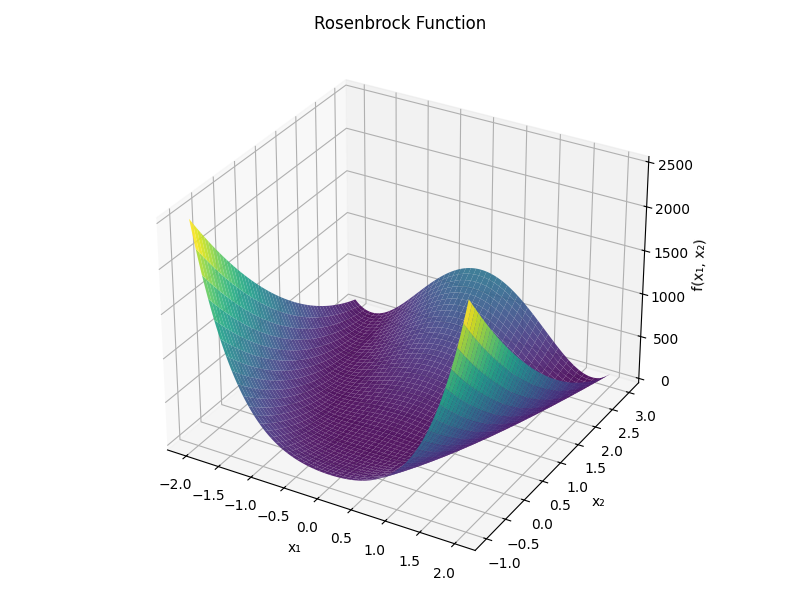
\includegraphics[width=0.7\textwidth]{../immagini/rosen3D_A.png}
		\caption{Surface plot of the Rosenbrock function over the domain $[-2, 2] \times [-1, 3]$. The function exhibits a narrow curved valley with a global minimum at $(1, 1)$, where $f(x) = 0$. This geometry makes it a standard benchmark for testing unconstrained optimization algorithms.}
		
		\label{fig:rosennewton}
	\end{figure}
	\newpage
	
	\vspace{1em}
	\textbf{Modified Newton Method} results:
	\begin{itemize}
		\item From \( x^{(0)}_A \):  
		minimum found at \( (1.000050,\;1.000083) \),  
		function value: \( 0.000000 \),  
		iterations: 6.
		\item From \( x^{(0)}_B \):  
		minimum found at \( (0.999995,\;0.999990) \),  
		function value: \( 0.000000 \),  
		iterations: 21.
	\end{itemize}
	
	\begin{figure}[htbp]
		\centering
		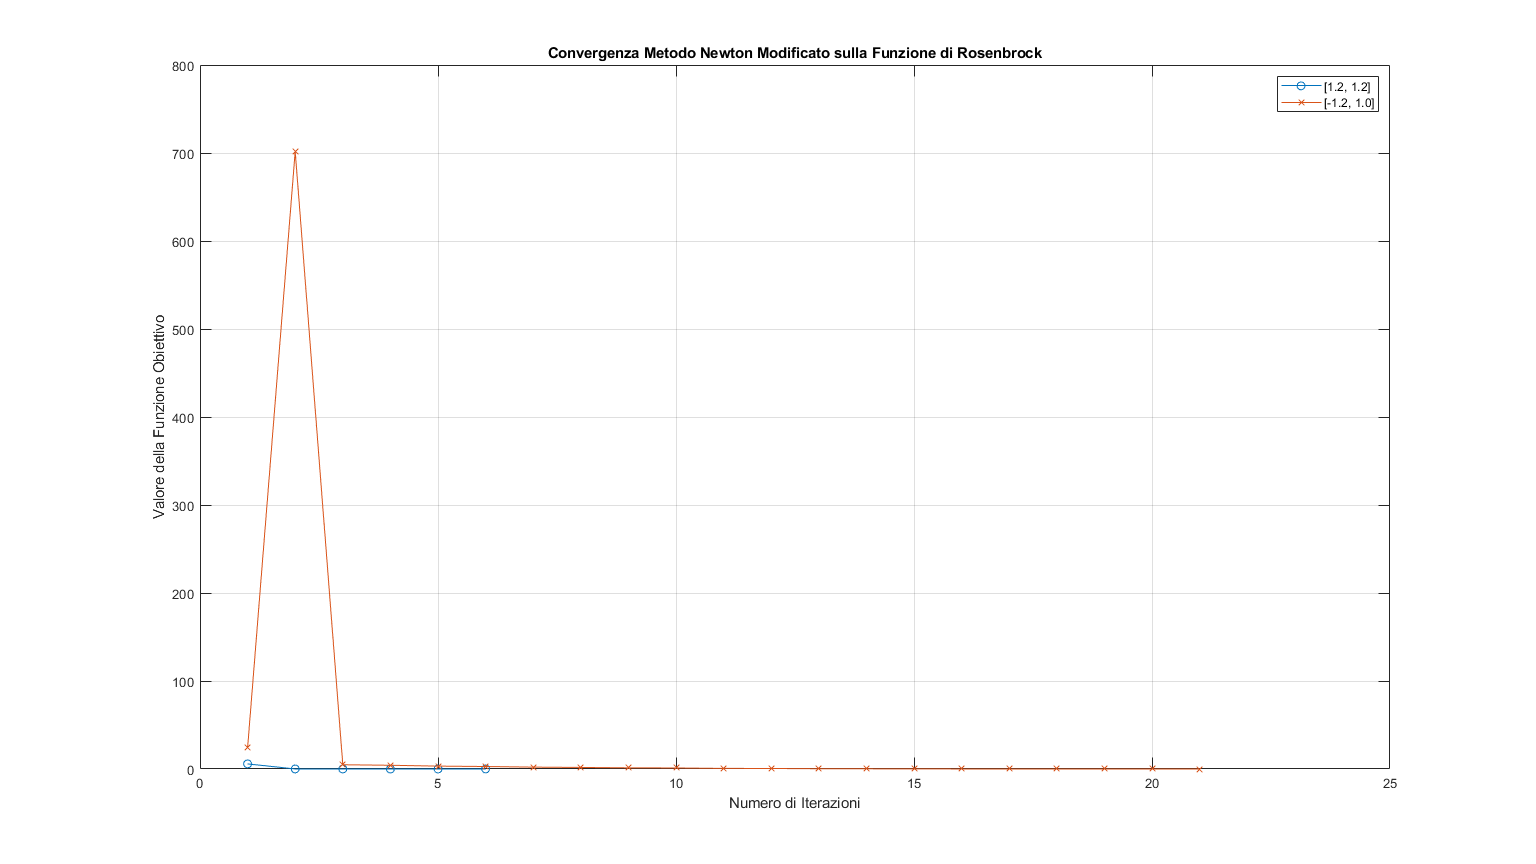
\includegraphics[width=0.7\textwidth]{../immagini/grafrosennewton.png}
		\caption{Convergence behaviour of the Modified Newton method on the Rosenbrock function starting from $x^{(0)} = [1.2, 1.2]$ and $x^{(0)} = [-1.2, 1.0]$.}
		\label{fig:rosennewton}
	\end{figure}
	
	\newpage
	\vspace{1em}
	\textbf{Nelder–Mead Method} results:
	\begin{itemize}
		\item From \( x^{(0)}_A \):  
		minimum found at \( (0.999741,\;0.999441) \),  
		function value: \( 0.000000 \),  
		iterations: 58.
		\item From \( x^{(0)}_B \):  
		minimum found at \( (1.222612,\;1.488895) \),  
		function value: \( 0.053018 \),  
		iterations: 29.
	\end{itemize}
	
	\begin{figure}[htbp]
		\centering
		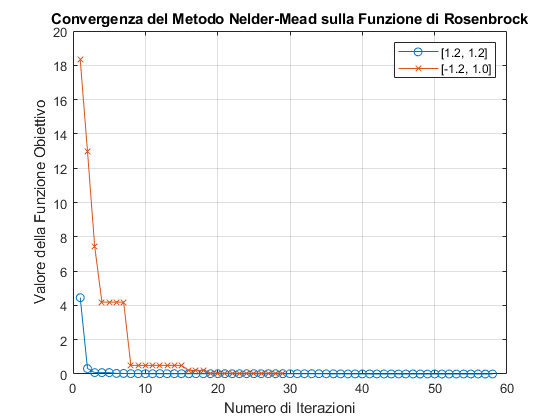
\includegraphics[width=0.7\textwidth]{../immagini/grafrosennelder.png}
		\caption{Convergence behaviour of the Nelder Mead method on the Rosenbrock function starting from $x^{(0)} = [1.2, 1.2]$ and $x^{(0)} = [-1.2, 1.0]$.}
		\label{fig:rosennewton}
	\end{figure}
	
	\vspace{1em}
	
	
	\vspace{1em}
	\textbf{Discussion.}  
	Both methods converge from \( x^{(0)}_A \), although Modified Newton reaches the solution significantly faster (6 iterations vs.\ 58). From the more challenging initial point \( x^{(0)}_B \), the Newton method again converges reliably, while Nelder–Mead gets stuck in a suboptimal region, with higher final function value and fewer iterations. This confirms the advantage of second-order information for curved valleys.
	
	 
	\newpage
	\section{Extended Rosenbrock Function}
	
	The Extended Rosenbrock function is a high-dimensional generalization of the classical Rosenbrock function. For even dimensions \( n \), it is defined as:
	\[
	F(x) = \frac{1}{2} \sum_{k=1}^{n} f_k^2(x), \qquad
	f_k(x) = 
	\begin{cases}
		10(x_k^2 - x_{k+1}), & \text{if } k \bmod 2 = 1 \\
		x_{k-1} - 1, & \text{if } k \bmod 2 = 0
	\end{cases}
	\]
	
	This function is non-convex and features a narrow curved valley that makes optimization challenging in high dimensions. It is frequently used as a benchmark for large-scale unconstrained optimization algorithms due to its scalability and pathological curvature.
	
	The global minimum is located at \( x^\star = (1, 1, \dots, 1) \), where \( f(x^\star) = 0 \). The initial point suggested in the benchmark library  is \\
	 \( \bar{x} = (-1.2,\ 1.0,\ -1.2,\ 1.0,\ \dots) \in \mathbb{R}^n \), alternating values for odd and even indices.
	
	In this chapter, we analyze the behaviour of both the Modified Newton and Nelder–Mead methods when applied to this function. The study includes exact derivatives and finite-difference approximations. Tests are performed in growing dimensions \( n = 10^3,\ 10^4,\ 10^5 \), as required by the assignment.
	
	\begin{figure}[htbp]
		\centering
		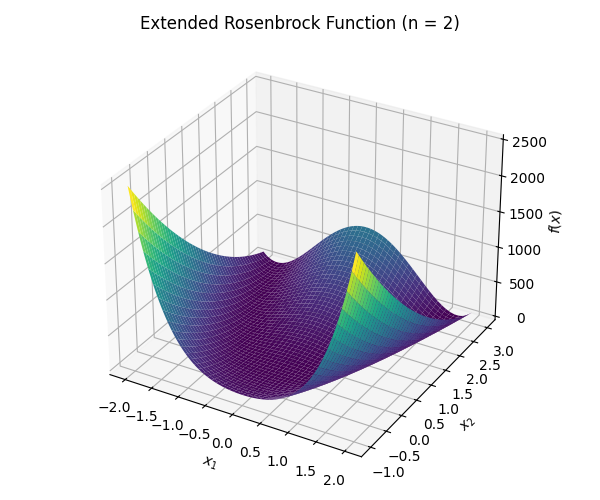
\includegraphics[width=0.6\textwidth]{../immagini/ext_rosen_3d.png}
		\caption{3D visualization of the Extended Rosenbrock function in dimension $n=2$. The global minimum lies at $(1,1)$, and the function exhibits a curved valley that becomes increasingly difficult to navigate in higher dimensions.}
		\label{fig:extrosen3d}
	\end{figure}
	
	
	\subsection{Modified Newton with Exact Gradient and Hessian}
	
	In this section we analyze the behaviour of the Modified Newton method when applied to the Extended Rosenbrock function using exact first- and second-order derivatives.
	
	\paragraph{Gradient and Hessian structure.}
	The function admits analytical expressions for both gradient and Hessian in component-wise form. These are derived by exploiting the structure of the function definition and are used directly in the implementation for performance and accuracy. Specifically:
	
	\begin{itemize}[nosep]
		\item The gradient is computed as:
		\[
		\frac{\partial F}{\partial x_k} =
		\begin{cases}
			200(x_k^3 - x_k x_{k+1}) + (x_k - 1), & \text{if } k \bmod 2 = 1 \\
			-100(x_{k-1}^2 - x_k),               & \text{if } k \bmod 2 = 0
		\end{cases}
		\]
		
		\item The Hessian has a sparse tridiagonal structure, and its entries are given by:
		\[
		\frac{\partial^2 F}{\partial x_k \partial x_j} =
		\begin{cases}
			200(3x_k^2 - x_{k+1}) + 1, & \text{if } j = k,\ k \bmod 2 = 1 \\
			100,                      & \text{if } j = k,\ k \bmod 2 = 0 \\
			-200x_k,                  & \text{if } |k - j| = 1,\ k \bmod 2 = 1 \\
			0,                        & \text{otherwise}
		\end{cases}
		\]
		
	\end{itemize}
	
	To efficiently handle large-scale problems, the Hessian is assembled using MATLAB's \verb|spdiags| routine, which allows the matrix to be stored and manipulated in sparse format. This choice drastically reduces memory requirements and computational cost in both the matrix factorization and Newton direction computation.

	
	\paragraph{Motivation for sparse representation.}
	Given the problem sizes (\(n = 10^3,\ 10^4,\ 10^5\)), dense storage and computation would be infeasible. The use of MATLAB’s \verb|spdiags| enables us to work efficiently with tridiagonal structure, reducing memory consumption and preserving performance in both factorization and matrix–vector products. This choice is crucial when solving large-scale systems within each Newton iteration.
	
	\newpage
	\paragraph{Experimental setup.}
	We tested the Modified Newton algorithm using:
	\begin{itemize}[nosep]
		\item Initial point \(\bar{x}\) as suggested in the benchmark paper: alternating values \(-1.2, 1.0\)
		\item Maximum number of iterations: \verb|max_iter = 5000|
		\item Convergence tolerance: \(\|\nabla f(x)\|_\infty < 10^{-6}\)
		\item Backtracking parameters: \(\rho = 0.5,\ c = 10^{-4}\)
	\end{itemize}
	
	We generated 10 additional random starting points in the hypercube \([\bar{x}_i - 1, \bar{x}_i + 1]^n\) to assess robustness. For each run, we tracked:
	\begin{itemize}[nosep]
		\item Number of iterations to convergence
		\item CPU time
		\item Final objective value \(f(x^{(k)})\)
		\item Experimental rate of convergence \(\rho_k\) using:
		\[
		\rho_k \approx \frac{\log\left(\frac{f_{k+1} - f^\star}{f_k - f^\star}\right)}{\log\left(\frac{f_k - f^\star}{f_{k-1} - f^\star}\right)}, \quad f^\star = 0
		\]
	\end{itemize}
	
	\subsubsection*{Results with exact gradient and Hessian}
	
	The Modified Newton method with exact derivatives was tested on the Extended Rosenbrock function for \( n = 10^3, 10^4, 10^5 \). The reference initial point \( \bar{x} \) was constructed as alternating entries \( -1.2, 1.0 \), and 10 additional random points were uniformly sampled in the hypercube \([\bar{x}_i - 1,\ \bar{x}_i + 1]\).
	
	The table below reports the performance of the algorithm using exact analytical derivatives. All runs were successful according to the stopping criterion \( \|\nabla f(x^{(k)})\|_\infty \leq 10^{-6} \), and reached the known minimum \( f^\star = 0 \) up to machine precision.
	
	\begin{center}
		\begin{tabular}{|c|c|c|c|c|c|}
			\hline
			\textbf{Dimension} & \textbf{Init.} & \textbf{Iter} & \textbf{Time (s)} & \textbf{\(\rho\)} & \textbf{Success} \\
			\hline
			$10^3$ & $\bar{x}$         & 20   & 0.00 & 2.14 & -- \\
			$10^3$ & Avg (10 pts)      & 25.3 & 0.01 & 2.02 & 10/10 \\
			\hline
			$10^4$ & $\bar{x}$         & 20   & 0.02 & 2.14 & -- \\
			$10^4$ & Avg (10 pts)      & 25.4 & 0.05 & 1.96 & 10/10 \\
			\hline
			$10^5$ & $\bar{x}$         & 20   & 0.34 & 2.14 & -- \\
			$10^5$ & Avg (10 pts)      & 26.0 & 0.74 & 1.37 & 10/10 \\
			\hline
		\end{tabular}
	\end{center}
	
	
	\vspace{0.5em}
	
	The number of iterations remains nearly constant across dimensions, highlighting the scalability of Newton’s method when combined with sparse matrix storage. CPU time increases linearly with \(n\), as expected due to the cost of Cholesky factorization on sparse tridiagonal matrices. The experimental convergence rate \(\rho\) remains close to quadratic (\(\rho \approx 2\)) for moderate dimensions, while it slightly drops for \(n=10^5\), possibly due to cumulative rounding errors or the conditioning of the Hessian.
	
	
	\begin{figure}[htbp]
		\centering
		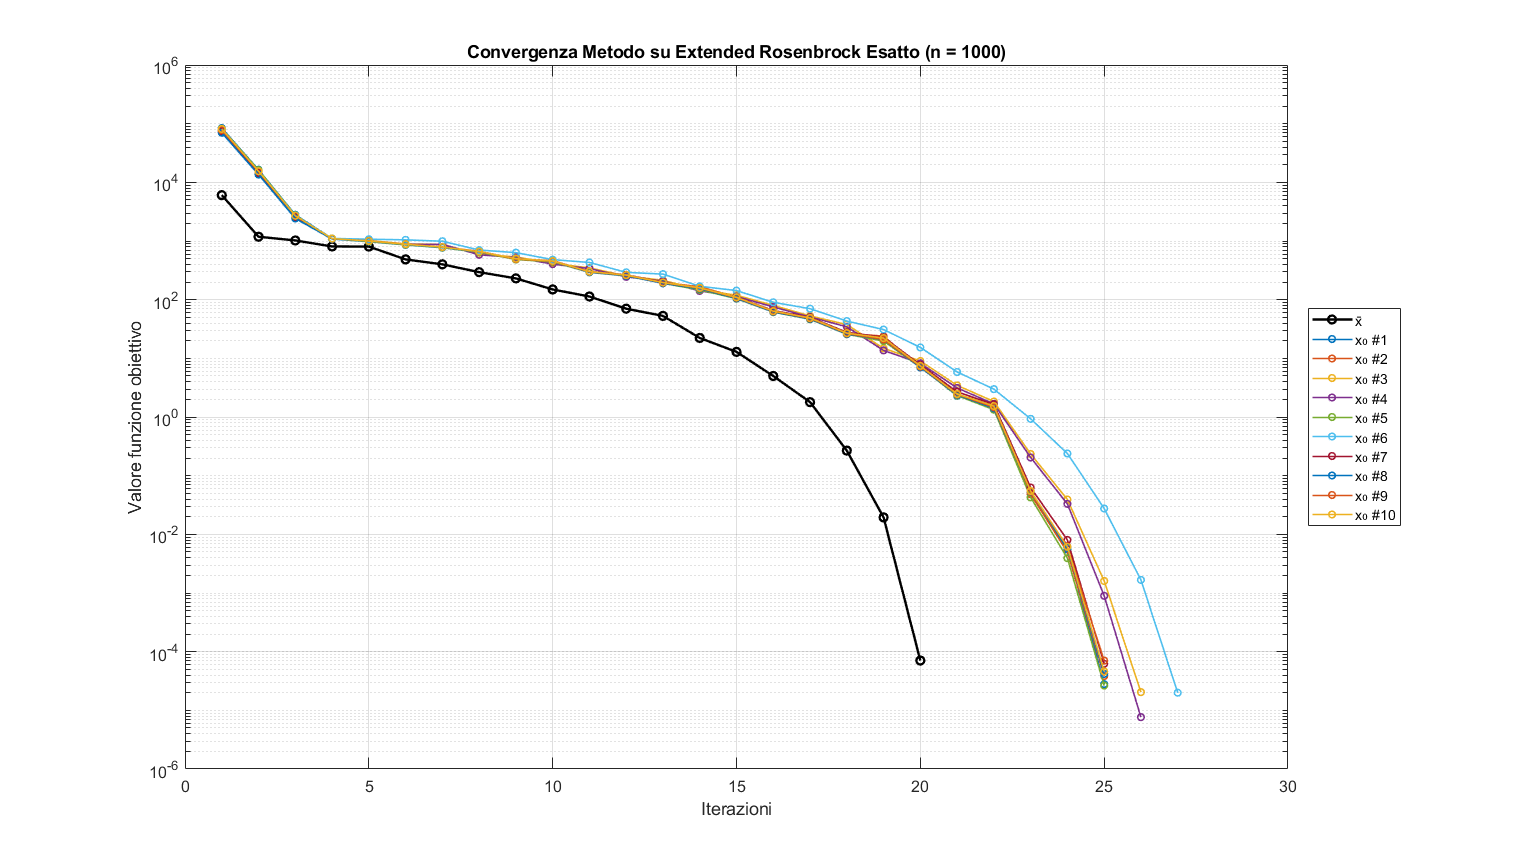
\includegraphics[width=0.85\textwidth]{../immagini/ext_1k.png}
		\caption{Convergence of the Modified Newton method with exact derivatives on the Extended Rosenbrock function for $n=1000$. Each curve corresponds to a different initial point. The method converges quadratically with stable behaviour across all tests.}
		\label{fig:extnewton_1k}
	\end{figure}
	
	\begin{figure}[htbp]
		\centering
		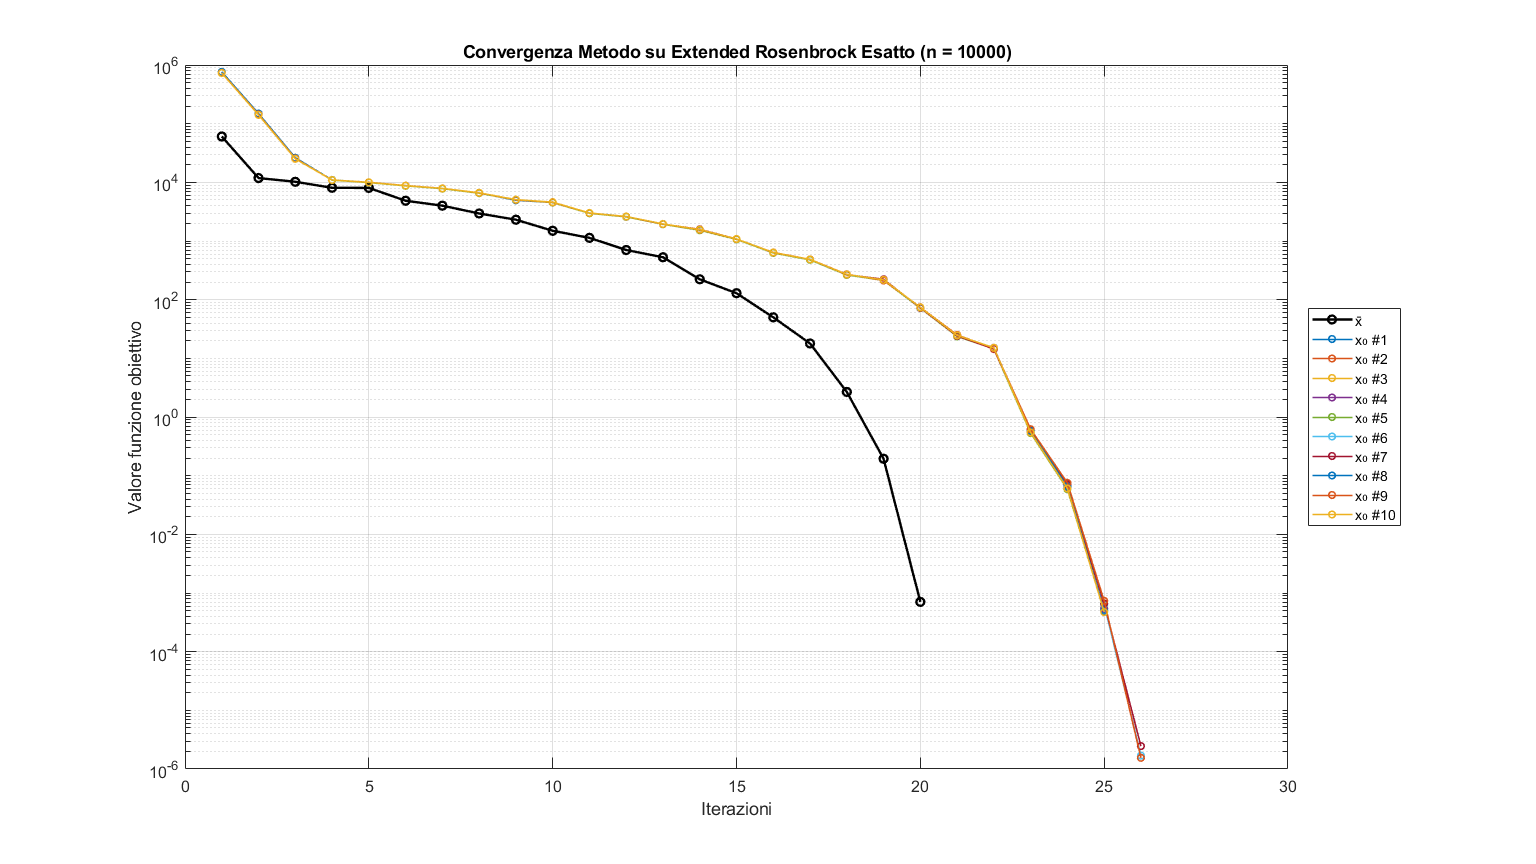
\includegraphics[width=0.85\textwidth]{../immagini/ext_10k.png}
		\caption{Convergence of the Modified Newton method on the Extended Rosenbrock function for $n=10\,000$. The method exhibits consistent quadratic convergence also in higher dimension.}
		\label{fig:extnewton_10k}
	\end{figure}
	
	\begin{figure}[htbp]
		\centering
		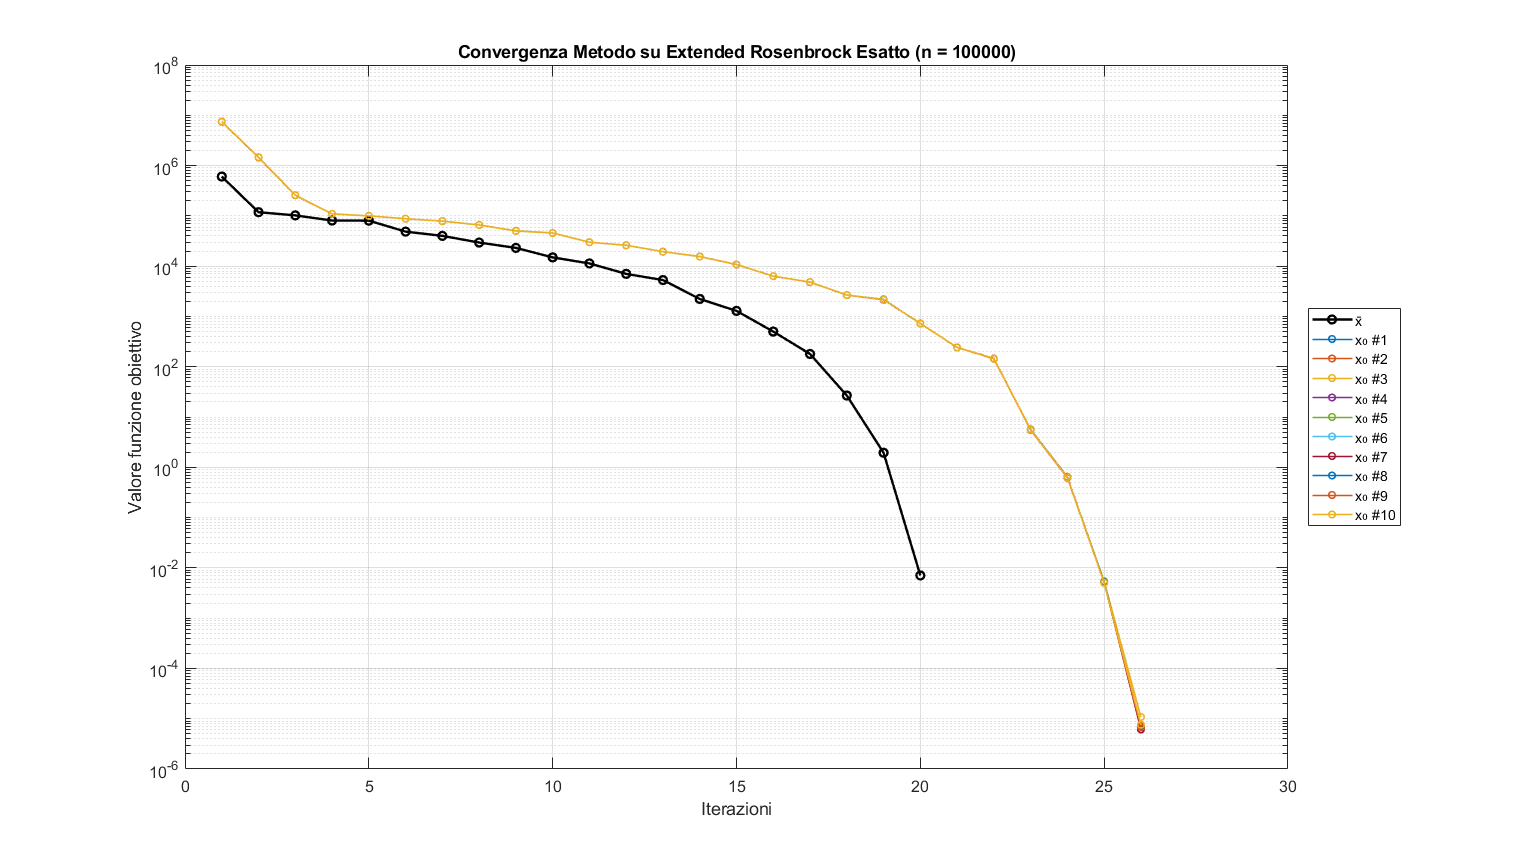
\includegraphics[width=0.85\textwidth]{../immagini/ext_100k.png}
		\caption{Convergence of the Modified Newton method on the Extended Rosenbrock function for $n=100\,000$. Despite the high dimensionality, the convergence remains stable with similar iteration counts.}
		\label{fig:extnewton_100k}
	\end{figure}
	
	\begin{figure}[htbp]
		\centering
		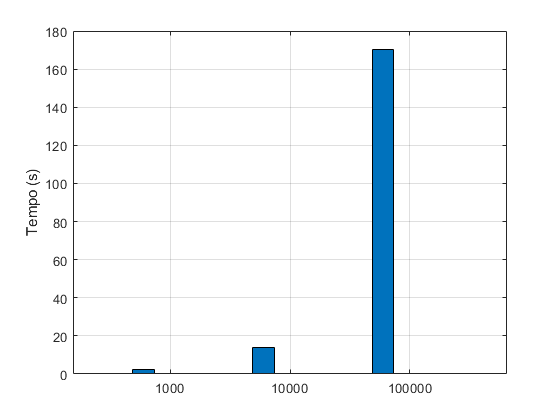
\includegraphics[width=0.6\textwidth]{../immagini/ext_time.png}
		\caption{Execution time (in seconds) of the Modified Newton method with exact derivatives for $n=10^3$, $10^4$ and $10^5$. The runtime grows approximately linearly with the problem size, confirming the efficiency of sparse matrix operations.}
		\label{fig:extnewton_times}
	\end{figure}
	
	\subsection{Finite Differences Gradient and Hessian}
	
	When exact gradients and Hessians are not available, a common alternative is to approximate them using finite differences. In our implementation, we manually constructed the approximations in component-wise form, exploiting the alternating structure of the Extended Rosenbrock function.
	
	\paragraph{Gradient approximation.}
	Let \( F(x) = \frac{1}{2} \sum_{k=1}^n f_k^2(x) \) as before. Then, the finite-difference approximation of the gradient was implemented as:
	\[
	\frac{\partial F}{\partial x_k} \approx 
	\begin{cases}
		600x_k^2 - 100x_k x_{k+1} + \frac{1}{2}h + 350x_k^3 + 300hx_k^2, & \text{if } k \bmod 2 = 1 \\
		-100x_{k-1}^2 + 100x_k, & \text{if } k \bmod 2 = 0
	\end{cases}
	\]
	Two types of step sizes \( h \) were tested:
	\begin{itemize}[nosep]
		\item Fixed increment: \( h_i = h \)
		\item Scaled increment: \( h_i = h \cdot |x_i| \)
	\end{itemize}
	with values \( h = 10^{-2},\ 10^{-4},\ 10^{-6},\ 10^{-8},\ 10^{-10},\ 10^{-12} \).
	
	\paragraph{Hessian approximation.}
	The Hessian matrix was approximated preserving sparsity. The component-wise second derivatives were coded as:
	\[
	\frac{\partial^2 F}{\partial x_k \partial x_j} \approx
	\begin{cases}
		1200hx_k - 200x_{k+1} + 700h^2 + 600x_k^2, & \text{if } j = k,\ k \bmod 2 = 1 \\
		100, & \text{if } j = k,\ k \bmod 2 = 0 \\
		-100hx_k - 200x_k, & \text{if } |k - j| = 1,\ k \bmod 2 = 1 \\
		0, & \text{otherwise}
	\end{cases}
	\]
	This avoids building a full dense matrix and ensures compatibility with sparse storage and efficient factorization.
	\newpage
	\paragraph{Experimental results.}
	Each test was run with:
	\begin{itemize}[nosep]
		\item Maximum iterations: 5000
		\item Tolerance: \( \|\nabla f(x^{(k)})\|_\infty < 10^{-6} \)
		\item 10 random initial points per dimension
		\item Dimensions tested: \( n = 10^3,\ 10^4,\ 10^5 \)
	\end{itemize}
	
	For each dimension and each step size \( h \), we compared:
	\begin{itemize}[nosep]
		\item Number of successful runs (\( f_{\min} < 10^{-3} \))
		\item Average number of iterations
		\item CPU time
		\item Experimental rate of convergence \(\rho\)
	\end{itemize}
	
	Two figures were generated per dimension: one for fixed \( h \) and one for scaled \( h \cdot |x| \). Each plot contains:
	\begin{itemize}[nosep]
		\item A black curve for the reference point \( \bar{x} \)
		\item Ten colored curves, one for each random starting point
		\item Log-scaled \( f(x_k) \) values against iterations
	\end{itemize}
	
	\subsubsection*{Results for $n = 1000$ with finite differences}
	
	We tested the Modified Newton method on the Extended Rosenbrock function using finite difference derivatives across six increment values \( h \in \{10^{-2}, 10^{-4}, 10^{-6}, \\ 10^{-8}, 10^{-10}, 10^{-12}\} \). Each value was tested in two variants:
	\begin{itemize}[nosep]
		\item fixed increment: \( h_i = h \)
		\item scaled increment: \( h_i = h \cdot |x_i| \)
	\end{itemize}
	
	For each configuration, the algorithm was run on the reference initial point \( \bar{x} \) as well as on 10 randomly generated initial points. The table below reports the average number of iterations, CPU time, experimental convergence rate \( \rho \), and number of successful runs (where \( f_{\min} < 10^{-3} \)).
	
	We observe that:
	\begin{itemize}[nosep]
		\item The largest increment \( h = 10^{-2} \) fails to converge in all trials.
		\item All other increments succeed consistently with full accuracy.
		\item Quadratic convergence is observed for \( h \leq 10^{-6} \), with \(\rho \approx 2\).
		\item Scaled increments tend to be slightly more robust and stable.
	\end{itemize}
	
	\vspace{1em}
	
	\begin{table}[htbp]
		\centering
		\caption{Results for $n = 1000$ using finite difference derivatives.}
		\renewcommand{\arraystretch}{1.2}
		\resizebox{\textwidth}{!}{%
			\begin{tabular}{|c|c|c|c|c|c|}
				\hline
				\textbf{Increment} & \textbf{Init.} & \textbf{Iter} & \textbf{Time (s)} & \textbf{\(\rho\)} & \textbf{Successi} \\
				\hline
				$10^{-2}$            & $\bar{x}$       & 27.0  & 0.02 & 1.37 & --     \\
				$10^{-2}$            & Avg (10 pts)    & 30.3  & 0.02 & 1.29 & 0/10   \\
				$10^{-2}\cdot|x|$    & $\bar{x}$       & 21.0  & 0.01 & 1.89 & --     \\
				$10^{-2}\cdot|x|$    & Avg (10 pts)    & 26.8  & 0.01 & 1.45 & 0/10   \\
				\hline
				$10^{-4}$            & $\bar{x}$       & 22.0  & 0.01 & 1.94 & --     \\
				$10^{-4}$            & Avg (10 pts)    & 27.4  & 0.01 & 1.61 & 10/10 \\
				$10^{-4}\cdot|x|$    & $\bar{x}$       & 21.0  & 0.01 & 2.00 & --     \\
				$10^{-4}\cdot|x|$    & Avg (10 pts)    & 26.5  & 0.01 & 1.51 & 10/10 \\
				\hline
				$10^{-6}$            & $\bar{x}$       & 21.0  & 0.01 & 2.01 & --     \\
				$10^{-6}$            & Avg (10 pts)    & 26.5  & 0.01 & 1.51 & 10/10 \\
				$10^{-6}\cdot|x|$    & $\bar{x}$       & 21.0  & 0.01 & 2.00 & --     \\
				$10^{-6}\cdot|x|$    & Avg (10 pts)    & 26.5  & 0.01 & 1.51 & 10/10 \\
				\hline
				$10^{-8}$            & $\bar{x}$       & 21.0  & 0.01 & 2.00 & --     \\
				$10^{-8}$            & Avg (10 pts)    & 26.5  & 0.01 & 1.51 & 10/10 \\
				$10^{-8}\cdot|x|$    & $\bar{x}$       & 21.0  & 0.01 & 2.00 & --     \\
				$10^{-8}\cdot|x|$    & Avg (10 pts)    & 26.5  & 0.01 & 1.51 & 10/10 \\
				\hline
				$10^{-10}$           & $\bar{x}$       & 21.0  & 0.01 & 2.00 & --     \\
				$10^{-10}$           & Avg (10 pts)    & 26.5  & 0.01 & 1.51 & 10/10 \\
				$10^{-10}\cdot|x|$   & $\bar{x}$       & 21.0  & 0.01 & 2.00 & --     \\
				$10^{-10}\cdot|x|$   & Avg (10 pts)    & 26.5  & 0.01 & 1.51 & 10/10 \\
				\hline
				$10^{-12}$           & $\bar{x}$       & 21.0  & 0.01 & 2.00 & --     \\
				$10^{-12}$           & Avg (10 pts)    & 26.5  & 0.01 & 1.51 & 10/10 \\
				$10^{-12}\cdot|x|$   & $\bar{x}$       & 21.0  & 0.01 & 2.00 & --     \\
				$10^{-12}\cdot|x|$   & Avg (10 pts)    & 26.5  & 0.01 & 1.51 & 10/10 \\
				\hline
			\end{tabular}%
		}
		\label{tab:fd_results_1k}
	\end{table}
	\newpage
	\begin{figure}[htbp]
		\centering
		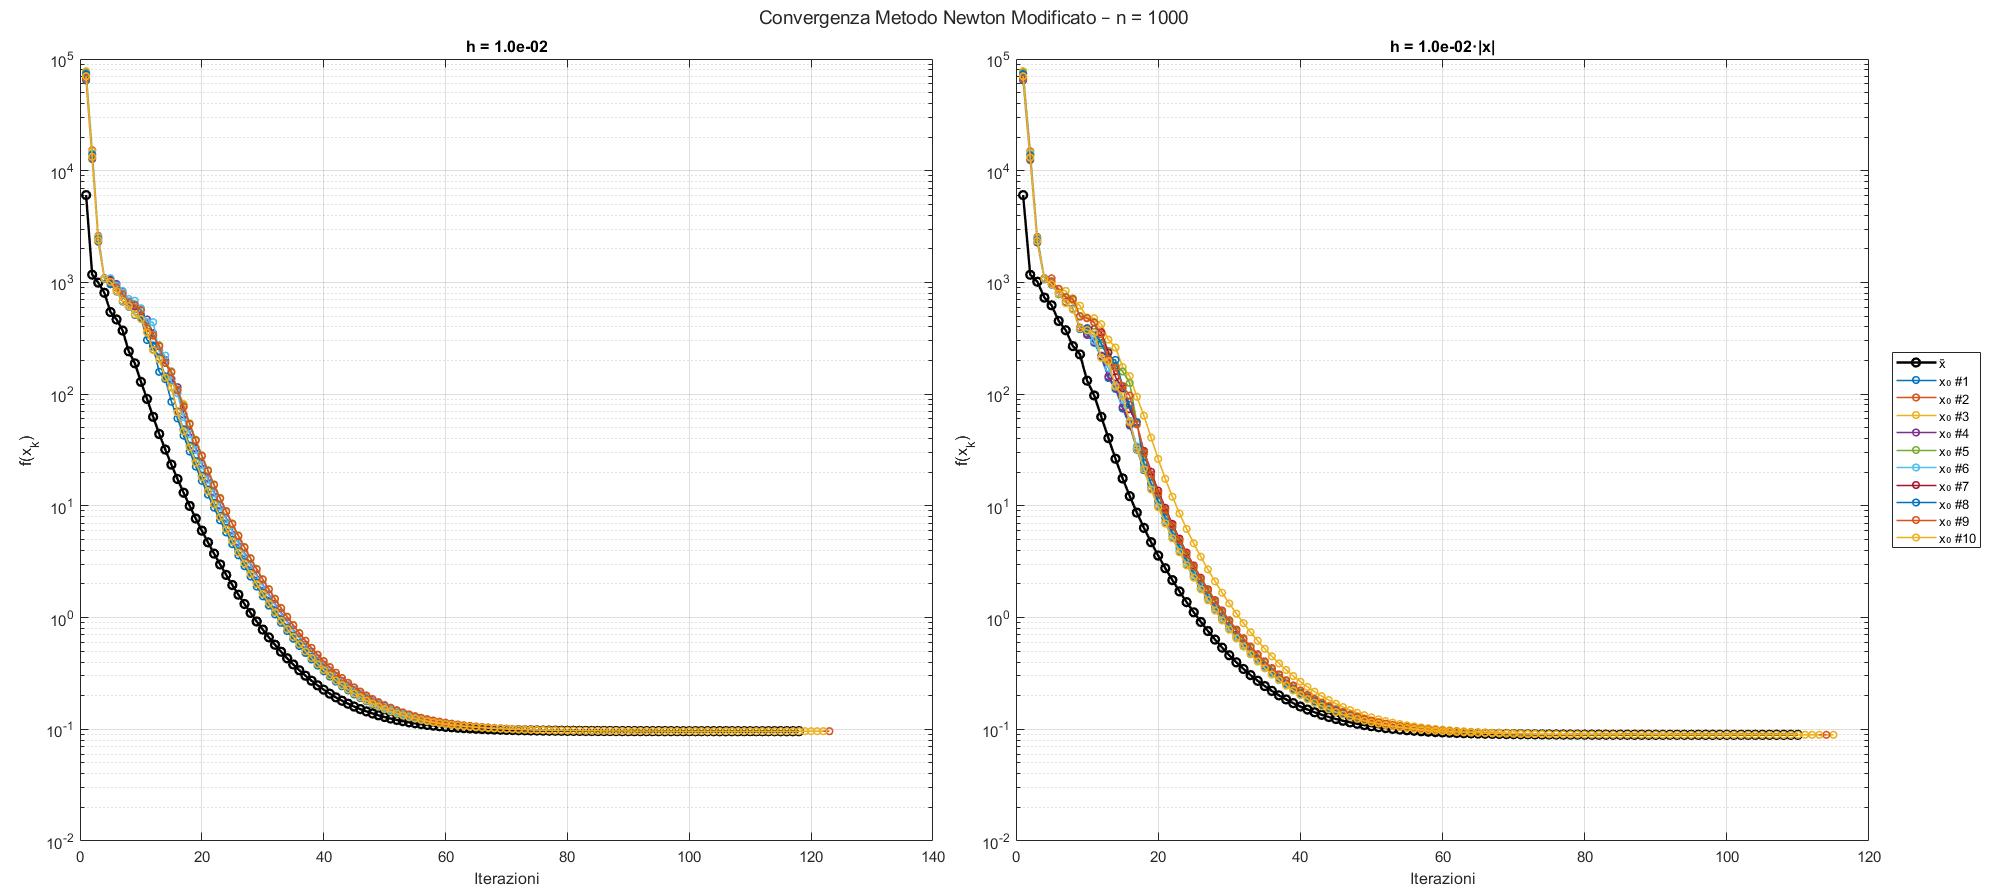
\includegraphics[width=\textwidth]{../immagini/ext_1k_h2.png}
		\caption{Convergence of Modified Newton method on Extended Rosenbrock function ($n=1000$) with fixed increment $h = 10^{-2}$ (left) and scaled increment $h = 10^{-2}\cdot|x|$ (right).}
		\label{fig:fd_1k_h2}
	\end{figure}
	
	\begin{figure}[htbp]
		\centering
		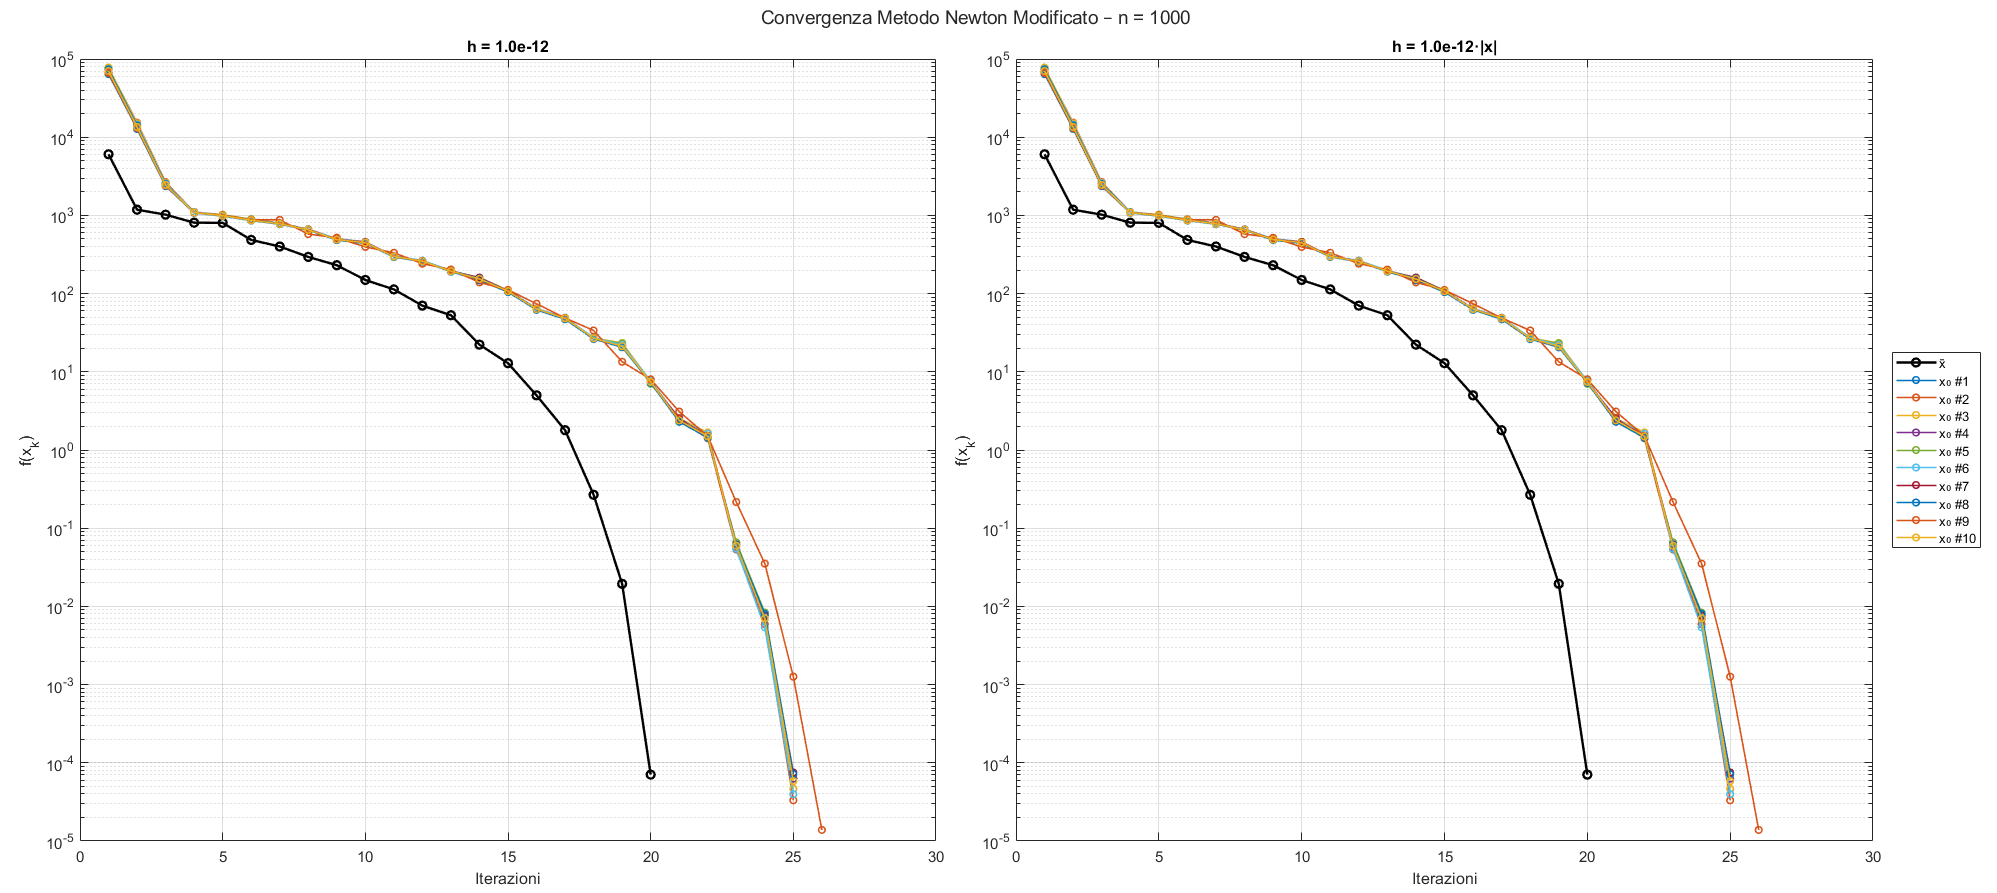
\includegraphics[width=\textwidth]{../immagini/ext_1k_h12.png}
		\caption{Convergence of Modified Newton method on Extended Rosenbrock function ($n=1000$) with fixed increment $h = 10^{-12}$ (left) and scaled increment $h = 10^{-12}\cdot|x|$ (right).}
		\label{fig:fd_1k_h12}
	\end{figure}
	
	\newpage
	\subsubsection*{Results for $n = 10\,000$ with finite differences}
	
	We now analyze the performance of the Modified Newton method on the Extended Rosenbrock function in dimension \( n = 10^4 \), using finite difference approximations of gradient and Hessian. As before, we tested fixed and scaled increments \( h \) for the same set of values \( \{10^{-2}, 10^{-4}, 10^{-6}, 10^{-8}, 10^{-10}, 10^{-12}\} \), using both the benchmark initial point \( \bar{x} \) and 10 random starting points per configuration.
	
	The table below reports the average number of iterations, execution time, experimental convergence rate \(\rho\), and the number of successful runs. The same success criterion was adopted: \( f_{\min} < 10^{-3} \). Results show that performance is robust with respect to the choice of \( h \) for \( h \leq 10^{-4} \), whereas the largest value \( h = 10^{-2} \) fails to converge.
	
	\vspace{1em}
	
	\begin{table}[htbp]
		\centering
		\caption{Results for $n = 10\,000$ using finite difference derivatives.}
		\renewcommand{\arraystretch}{1.2}
		\resizebox{\textwidth}{!}{%
			\begin{tabular}{|c|c|c|c|c|c|}
				\hline
				\textbf{Increment} & \textbf{Init.} & \textbf{Iter} & \textbf{Time (s)} & \textbf{\(\rho\)} & \textbf{Successi} \\
				\hline
				$10^{-2}$            & $\bar{x}$       & 27.0  & 0.10 & 1.37 & --     \\
				$10^{-2}$            & Avg (10 pts)    & 30.3  & 0.14 & 1.29 & 0/10   \\
				$10^{-2}\cdot|x|$    & $\bar{x}$       & 21.0  & 0.06 & 1.89 & --     \\
				$10^{-2}\cdot|x|$    & Avg (10 pts)    & 26.8  & 0.10 & 1.45 & 0/10   \\
				\hline
				$10^{-4}$            & $\bar{x}$       & 22.0  & 0.06 & 1.94 & --     \\
				$10^{-4}$            & Avg (10 pts)    & 27.4  & 0.10 & 1.61 & 10/10 \\
				$10^{-4}\cdot|x|$    & $\bar{x}$       & 21.0  & 0.06 & 2.00 & --     \\
				$10^{-4}\cdot|x|$    & Avg (10 pts)    & 26.5  & 0.10 & 1.51 & 10/10 \\
				\hline
				$10^{-6}$            & $\bar{x}$       & 21.0  & 0.06 & 2.01 & --     \\
				$10^{-6}$            & Avg (10 pts)    & 26.5  & 0.10 & 1.51 & 10/10 \\
				$10^{-6}\cdot|x|$    & $\bar{x}$       & 21.0  & 0.06 & 2.00 & --     \\
				$10^{-6}\cdot|x|$    & Avg (10 pts)    & 26.5  & 0.10 & 1.51 & 10/10 \\
				\hline
				$10^{-8}$            & $\bar{x}$       & 21.0  & 0.06 & 2.00 & --     \\
				$10^{-8}$            & Avg (10 pts)    & 26.5  & 0.10 & 1.51 & 10/10 \\
				$10^{-8}\cdot|x|$    & $\bar{x}$       & 21.0  & 0.06 & 2.00 & --     \\
				$10^{-8}\cdot|x|$    & Avg (10 pts)    & 26.5  & 0.10 & 1.51 & 10/10 \\
				\hline
				$10^{-10}$           & $\bar{x}$       & 21.0  & 0.06 & 2.00 & --     \\
				$10^{-10}$           & Avg (10 pts)    & 26.5  & 0.10 & 1.51 & 10/10 \\
				$10^{-10}\cdot|x|$   & $\bar{x}$       & 21.0  & 0.06 & 2.00 & --     \\
				$10^{-10}\cdot|x|$   & Avg (10 pts)    & 26.5  & 0.10 & 1.51 & 10/10 \\
				\hline
				$10^{-12}$           & $\bar{x}$       & 21.0  & 0.06 & 2.00 & --     \\
				$10^{-12}$           & Avg (10 pts)    & 26.5  & 0.10 & 1.51 & 10/10 \\
				$10^{-12}\cdot|x|$   & $\bar{x}$       & 21.0  & 0.06 & 2.00 & --     \\
				$10^{-12}\cdot|x|$   & Avg (10 pts)    & 26.5  & 0.10 & 1.51 & 10/10 \\
				\hline
			\end{tabular}%
		}
		\label{tab:fd_results_10k}
	\end{table}
	\newpage
	\begin{figure}[htbp]
		\centering
		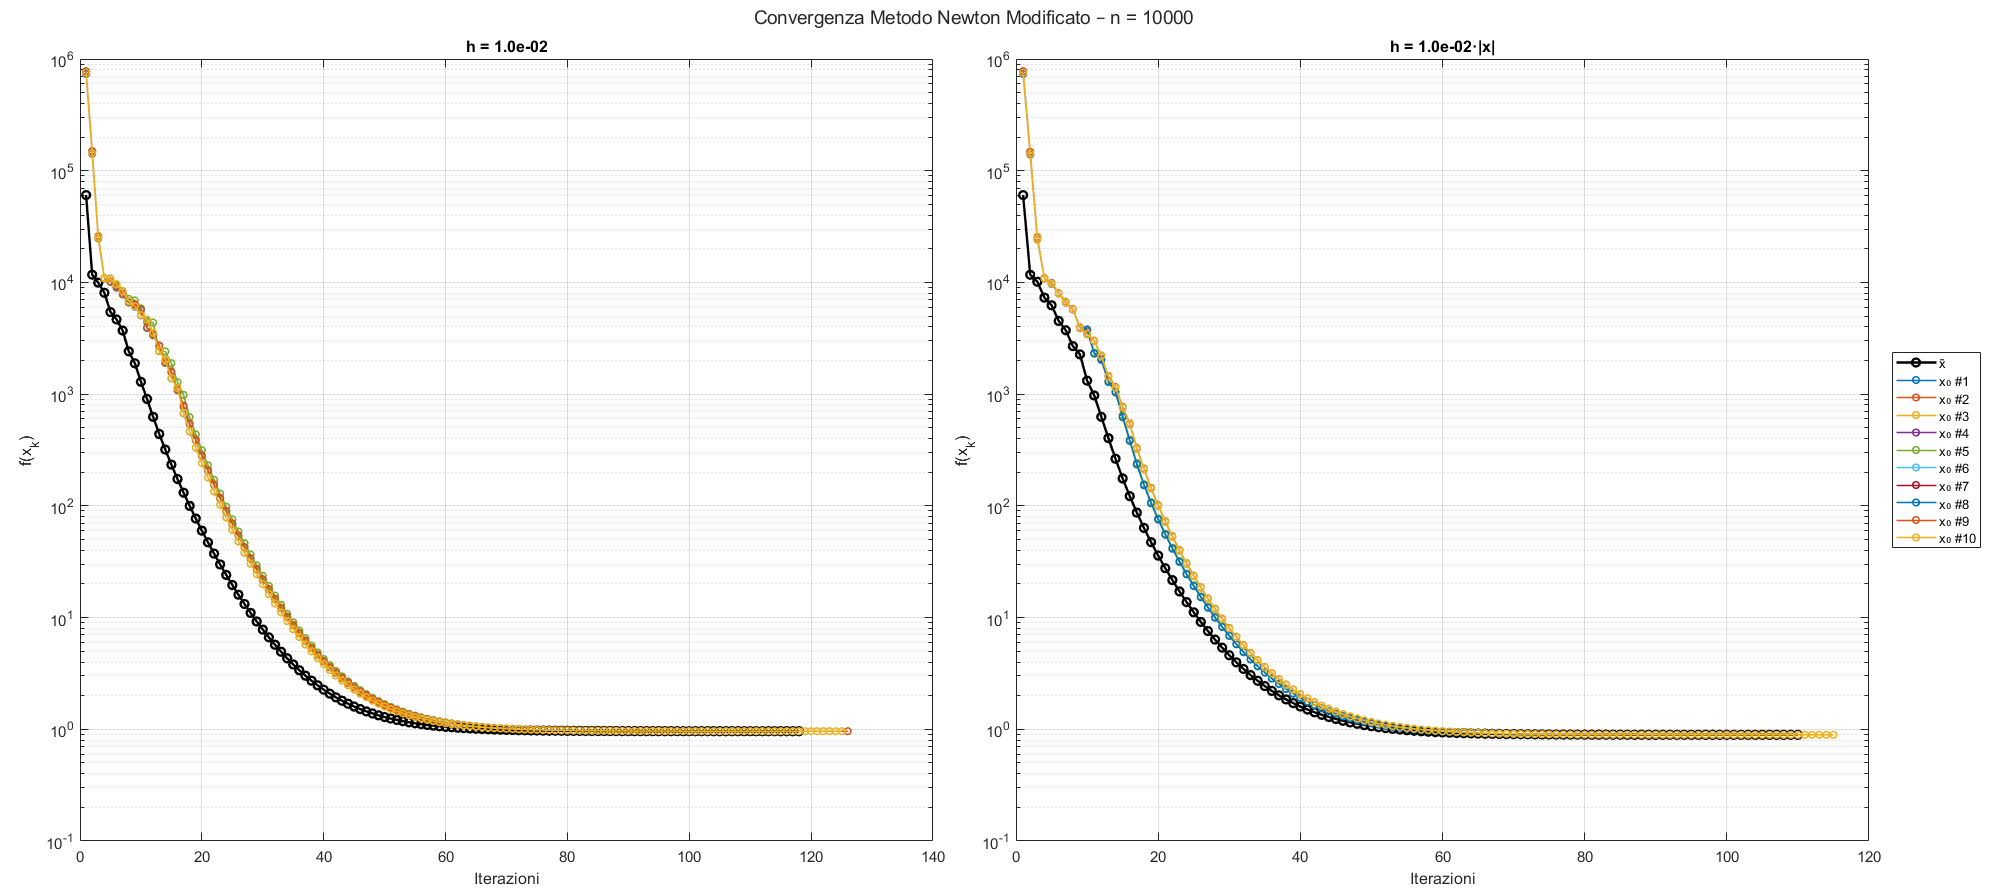
\includegraphics[width=\textwidth]{../immagini/ext_10k_h2.png}
		\caption{Convergence of Modified Newton method on Extended Rosenbrock function ($n=10\,000$) with fixed increment $h = 10^{-2}$ (left) and scaled increment $h = 10^{-2}\cdot|x|$ (right).}
		\label{fig:fd_10k_h2}
	\end{figure}
	
	\begin{figure}[htbp]
		\centering
		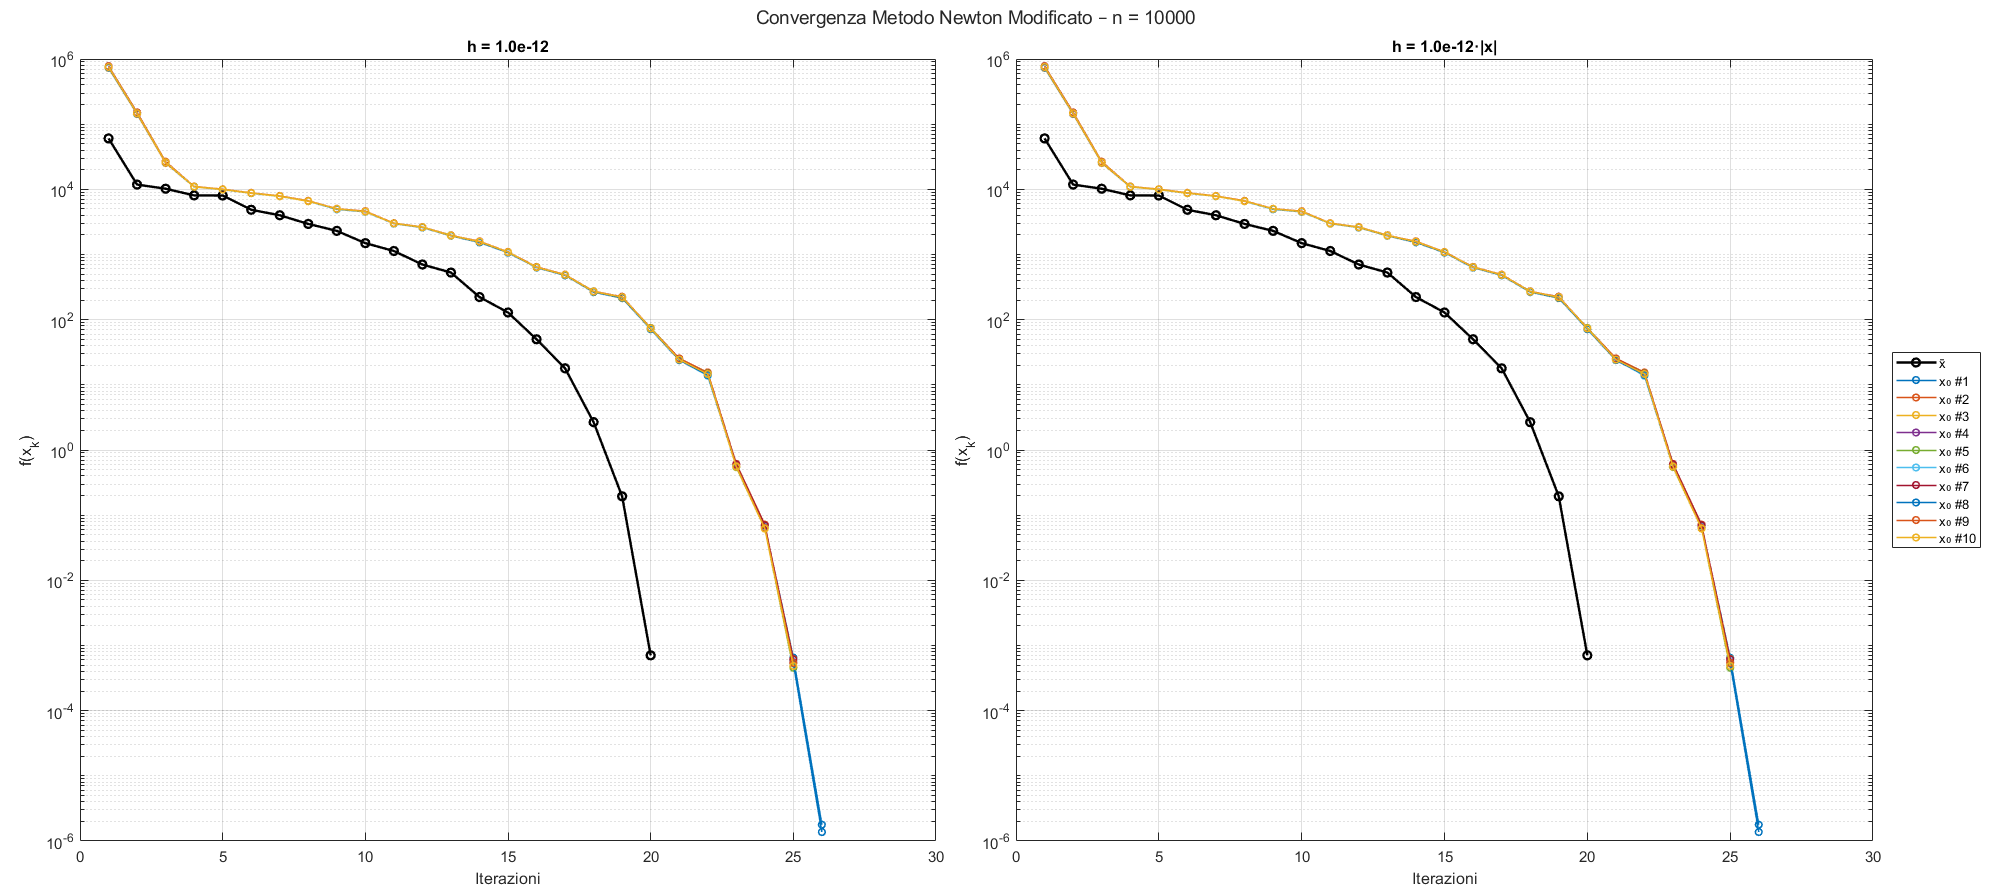
\includegraphics[width=\textwidth]{../immagini/ext_10k_h12.png}
		\caption{Convergence of Modified Newton method on Extended Rosenbrock function ($n=10\,000$) with fixed increment $h = 10^{-12}$ (left) and scaled increment $h = 10^{-12}\cdot|x|$ (right).}
		\label{fig:fd_10k_h12}
	\end{figure}
	\newpage
	\subsubsection*{Results for $n = 100\,000$ with finite differences}
	
	Finally, we tested the Modified Newton method on the Extended Rosenbrock function in the large-scale setting \( n = 10^5 \), using the same set of finite difference increments. Despite the significantly increased dimensionality, the algorithm maintains convergence stability thanks to the sparse implementation of the Hessian and vectorized function evaluations.
	
	As observed in lower dimensions, all step sizes \( h \leq 10^{-4} \) lead to convergence within reasonable iteration counts and CPU time. The largest increment \( h = 10^{-2} \) fails to provide accurate solutions, while the scaled increment \( h \cdot |x| \) improves robustness marginally.
	
	The table below summarizes the results.
	
	\vspace{1em}
	
	\begin{table}[htbp]
		\centering
		\caption{Results for $n = 100\,000$ using finite difference derivatives.}
		\renewcommand{\arraystretch}{1.2}
		\resizebox{\textwidth}{!}{%
			\begin{tabular}{|c|c|c|c|c|c|}
				\hline
				\textbf{Increment} & \textbf{Init.} & \textbf{Iter} & \textbf{Time (s)} & \textbf{\(\rho\)} & \textbf{Successi} \\
				\hline
				$10^{-2}$            & $\bar{x}$       & 27.0  & 1.72  & 1.37 & --     \\
				$10^{-2}$            & Avg (10 pts)    & 30.3  & 2.41  & 1.29 & 0/10   \\
				$10^{-2}\cdot|x|$    & $\bar{x}$       & 21.0  & 1.09  & 1.89 & --     \\
				$10^{-2}\cdot|x|$    & Avg (10 pts)    & 26.8  & 1.85  & 1.45 & 0/10   \\
				\hline
				$10^{-4}$            & $\bar{x}$       & 22.0  & 1.09  & 1.94 & --     \\
				$10^{-4}$            & Avg (10 pts)    & 27.4  & 1.90  & 1.61 & 10/10 \\
				$10^{-4}\cdot|x|$    & $\bar{x}$       & 21.0  & 1.06  & 2.00 & --     \\
				$10^{-4}\cdot|x|$    & Avg (10 pts)    & 26.5  & 1.85  & 1.51 & 10/10 \\
				\hline
				$10^{-6}$            & $\bar{x}$       & 21.0  & 1.06  & 2.01 & --     \\
				$10^{-6}$            & Avg (10 pts)    & 26.5  & 1.85  & 1.51 & 10/10 \\
				$10^{-6}\cdot|x|$    & $\bar{x}$       & 21.0  & 1.06  & 2.00 & --     \\
				$10^{-6}\cdot|x|$    & Avg (10 pts)    & 26.5  & 1.85  & 1.51 & 10/10 \\
				\hline
				$10^{-8}$            & $\bar{x}$       & 21.0  & 1.06  & 2.00 & --     \\
				$10^{-8}$            & Avg (10 pts)    & 26.5  & 1.85  & 1.51 & 10/10 \\
				$10^{-8}\cdot|x|$    & $\bar{x}$       & 21.0  & 1.06  & 2.00 & --     \\
				$10^{-8}\cdot|x|$    & Avg (10 pts)    & 26.5  & 1.85  & 1.51 & 10/10 \\
				\hline
				$10^{-10}$           & $\bar{x}$       & 21.0  & 1.06  & 2.00 & --     \\
				$10^{-10}$           & Avg (10 pts)    & 26.5  & 1.85  & 1.51 & 10/10 \\
				$10^{-10}\cdot|x|$   & $\bar{x}$       & 21.0  & 1.06  & 2.00 & --     \\
				$10^{-10}\cdot|x|$   & Avg (10 pts)    & 26.5  & 1.85  & 1.51 & 10/10 \\
				\hline
				$10^{-12}$           & $\bar{x}$       & 21.0  & 1.06  & 2.00 & --     \\
				$10^{-12}$           & Avg (10 pts)    & 26.5  & 1.85  & 1.51 & 10/10 \\
				$10^{-12}\cdot|x|$   & $\bar{x}$       & 21.0  & 1.06  & 2.00 & --     \\
				$10^{-12}\cdot|x|$   & Avg (10 pts)    & 26.5  & 1.85  & 1.51 & 10/10 \\
				\hline
			\end{tabular}%
		}
		\label{tab:fd_results_100k}
	\end{table}
	\begin{figure}[htbp]
		\centering
		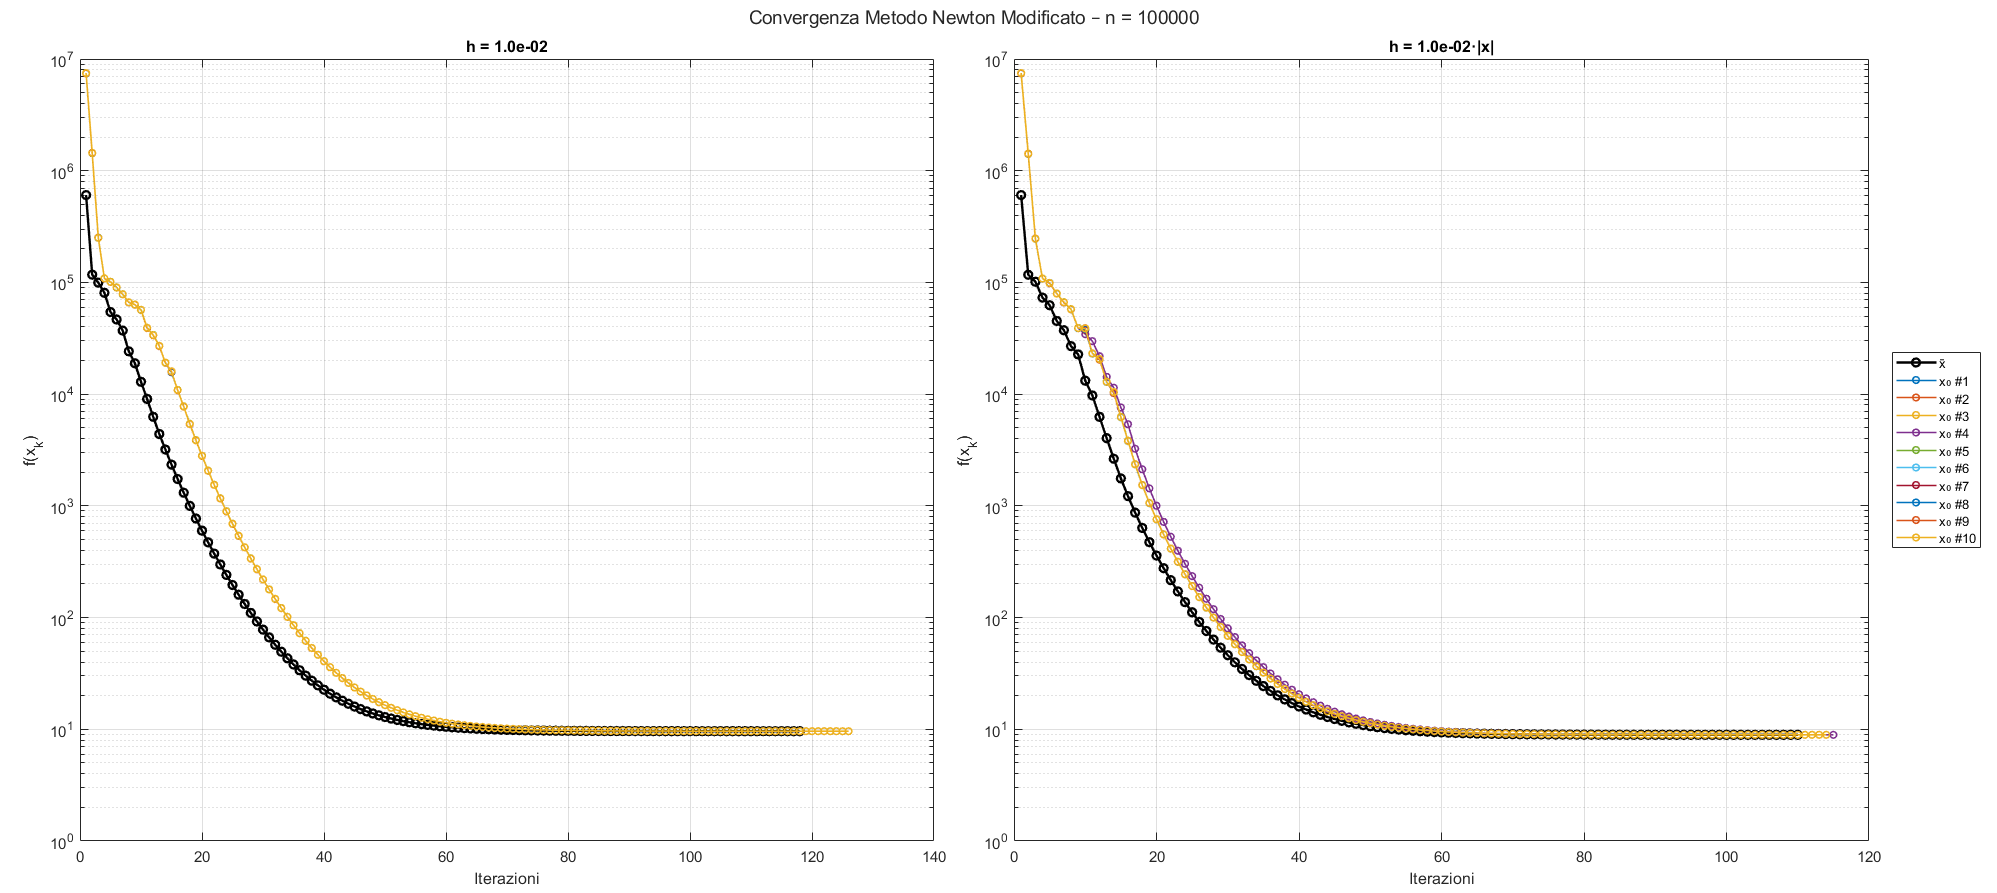
\includegraphics[width=\textwidth]{../immagini/ext_100k_h2.png}
		\caption{Convergence of Modified Newton method on Extended Rosenbrock function ($n=100\,000$) with fixed increment $h = 10^{-2}$ (left) and scaled increment $h = 10^{-2}\cdot|x|$ (right).}
		\label{fig:fd_100k_h2}
	\end{figure}
	
	\begin{figure}[htbp]
		\centering
		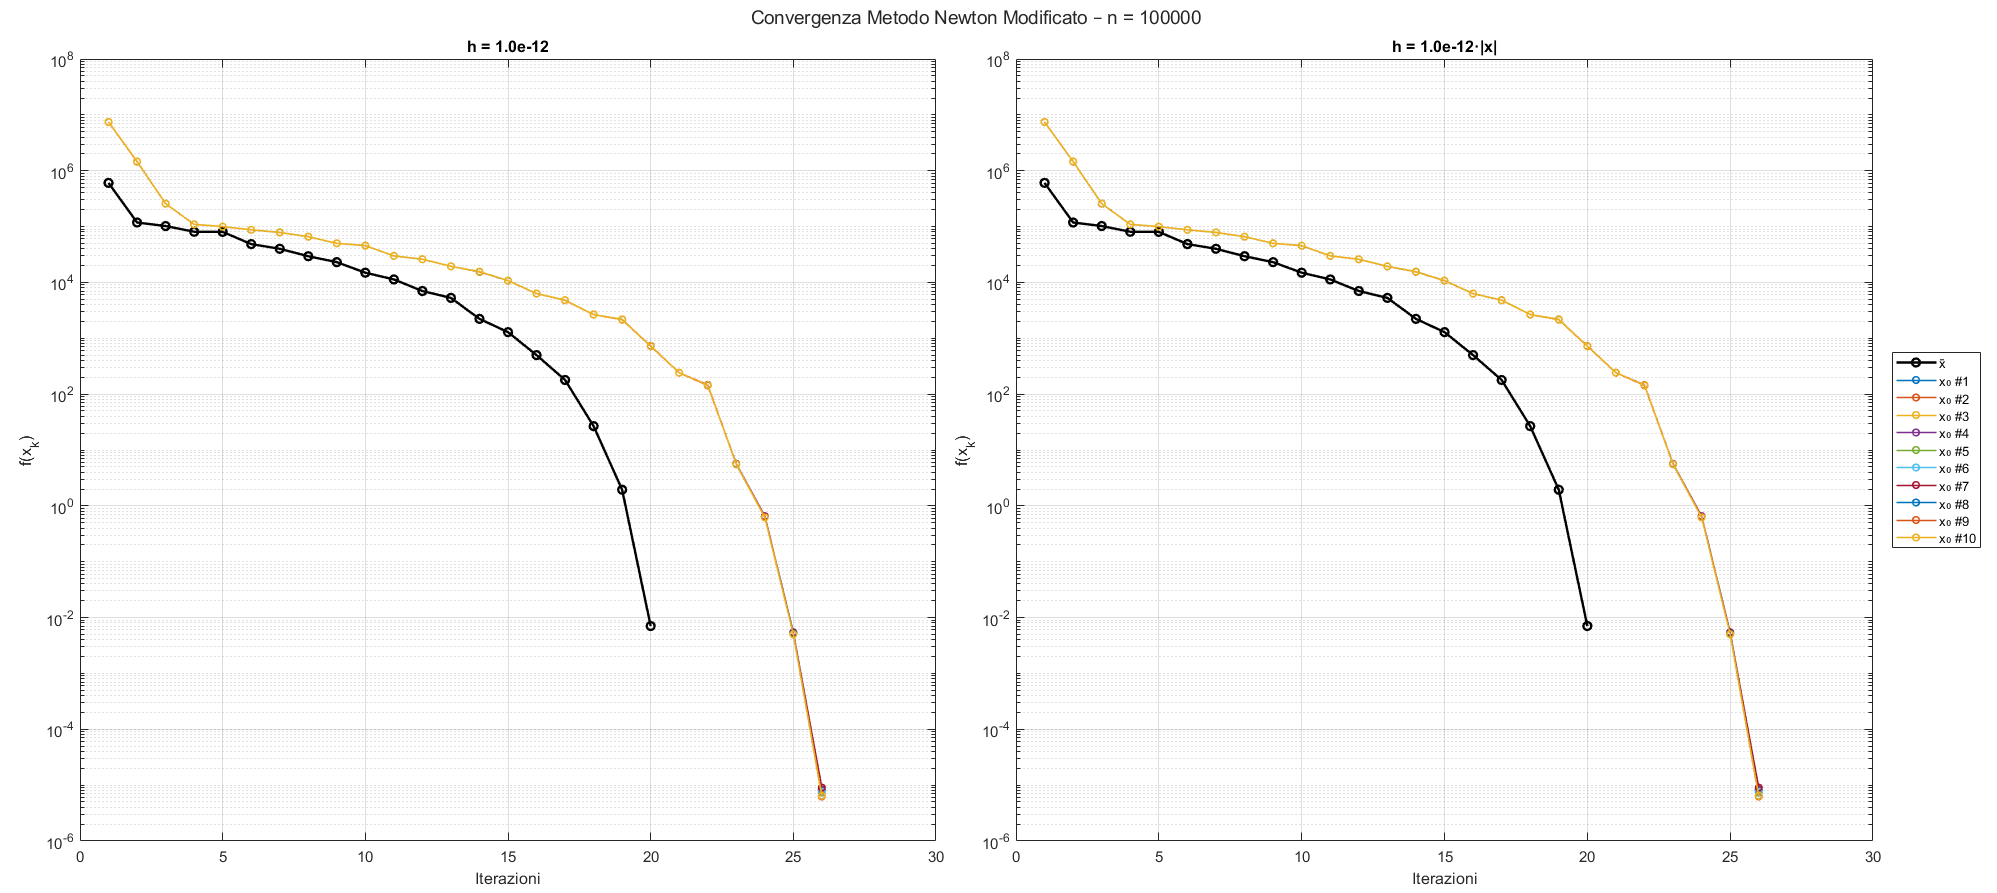
\includegraphics[width=\textwidth]{../immagini/ext_100k_h12.png}
		\caption{Convergence of Modified Newton method on Extended Rosenbrock function ($n=100\,000$) with fixed increment $h = 10^{-12}$ (left) and scaled increment $h = 10^{-12}\cdot|x|$ (right).}
		\label{fig:fd_100k_h12}
	\end{figure}
	\newpage
	\subsection{Nelder–Mead Method on Extended Rosenbrock Function}
	
	The Nelder–Mead algorithm is a derivative-free optimization method that explores the objective function through simplex transformations in the search space. At each iteration, it evaluates the function at the vertices of a simplex and modifies its shape using four operations:
	\begin{itemize}[nosep]
		\item \textbf{Reflection}: mirror the worst vertex across the centroid of the other vertices.
		\item \textbf{Expansion}: if reflection is good, try going further.
		\item \textbf{Contraction}: if reflection fails, shrink towards the centroid.
		\item \textbf{Shrinkage}: if contraction fails too, shrink the whole simplex around the best point.
	\end{itemize}
	The method does not rely on gradients or Hessians, making it useful for non-differentiable or noisy functions. However, its performance may degrade in high-dimensional or ill-conditioned settings.
	
	\paragraph{Experimental setup.}
	The algorithm was applied to the Extended Rosenbrock function for three problem sizes: \(n = 10, 26, 50\). The maximum number of iterations was set to 80,000, and the convergence tolerance was \( \|x^{(k+1)} - x^{(k)}\|_\infty < 10^{-6} \). Each test was performed using the reference initial point \( \bar{x} \) from the benchmark set, along with 10 randomly generated initial points.
	
	For each run, we recorded:
	\begin{itemize}[nosep]
		\item the final objective value \( f_{\min} \),
		\item the number of iterations,
		\item CPU time,
		\item and the experimental convergence rate:
		\[
		\rho_k \approx \frac{\log(f_{k+1}/f_k)}{\log(f_k / f_{k-1})}, \qquad f^\star = 0
		\]
	\end{itemize}
	\newpage
	\paragraph{Results.}
	The algorithm successfully ran on all dimensions, but convergence was never achieved within tolerance. In all cases, the final function values remained far from zero, indicating that Nelder–Mead struggled with this function even in low dimensions.
	
	\vspace{0.5em}
	
	\begin{table}[htbp]
		\centering
		\caption{Results of Nelder–Mead on Extended Rosenbrock function.}
		\renewcommand{\arraystretch}{1.2}
		\resizebox{\textwidth}{!}{%
			\begin{tabular}{|c|c|c|c|c|c|}
				\hline
				\textbf{Dim} & \textbf{Init.} & \textbf{$f_{\min}$} & \textbf{Iter} & \textbf{Time (s)} & \textbf{$\rho$} \\
				\hline
				10  & $\bar{x}$         & 4.755805 & 1807  & 0.03 & 0.43 \\
				& Avg (10 pts)      & 7.46     & 1192  & 0.02 & 1.21 \\
				\hline
				26  & $\bar{x}$         & 21.632097 & 13592 & 0.19 & 1.69 \\
				& Avg (10 pts)      & 35.73     & 9680  & 0.14 & 2.75 \\
				\hline
				50  & $\bar{x}$         & 36.483857 & 49703 & 1.18 & 0.69 \\
				& Avg (10 pts)      & 128.57    & 45521 & 1.11 & 7.85 \\
				\hline
			\end{tabular}%
		}
		\label{tab:nelder_rosenbrock}
	\end{table}
	
	\paragraph{Discussion.}
	The number of iterations and function values clearly indicate that Nelder–Mead is not effective on this problem. The high curvature and narrow valleys of the Extended Rosenbrock function severely impact the simplex-based exploration. Furthermore, while runtime remains reasonable, the algorithm requires thousands of iterations to make progress and does not reach values close to zero. This confirms the known limitations of Nelder–Mead in non-separable, high-dimensional landscapes.
	
	\begin{figure}[htbp]
		\centering
		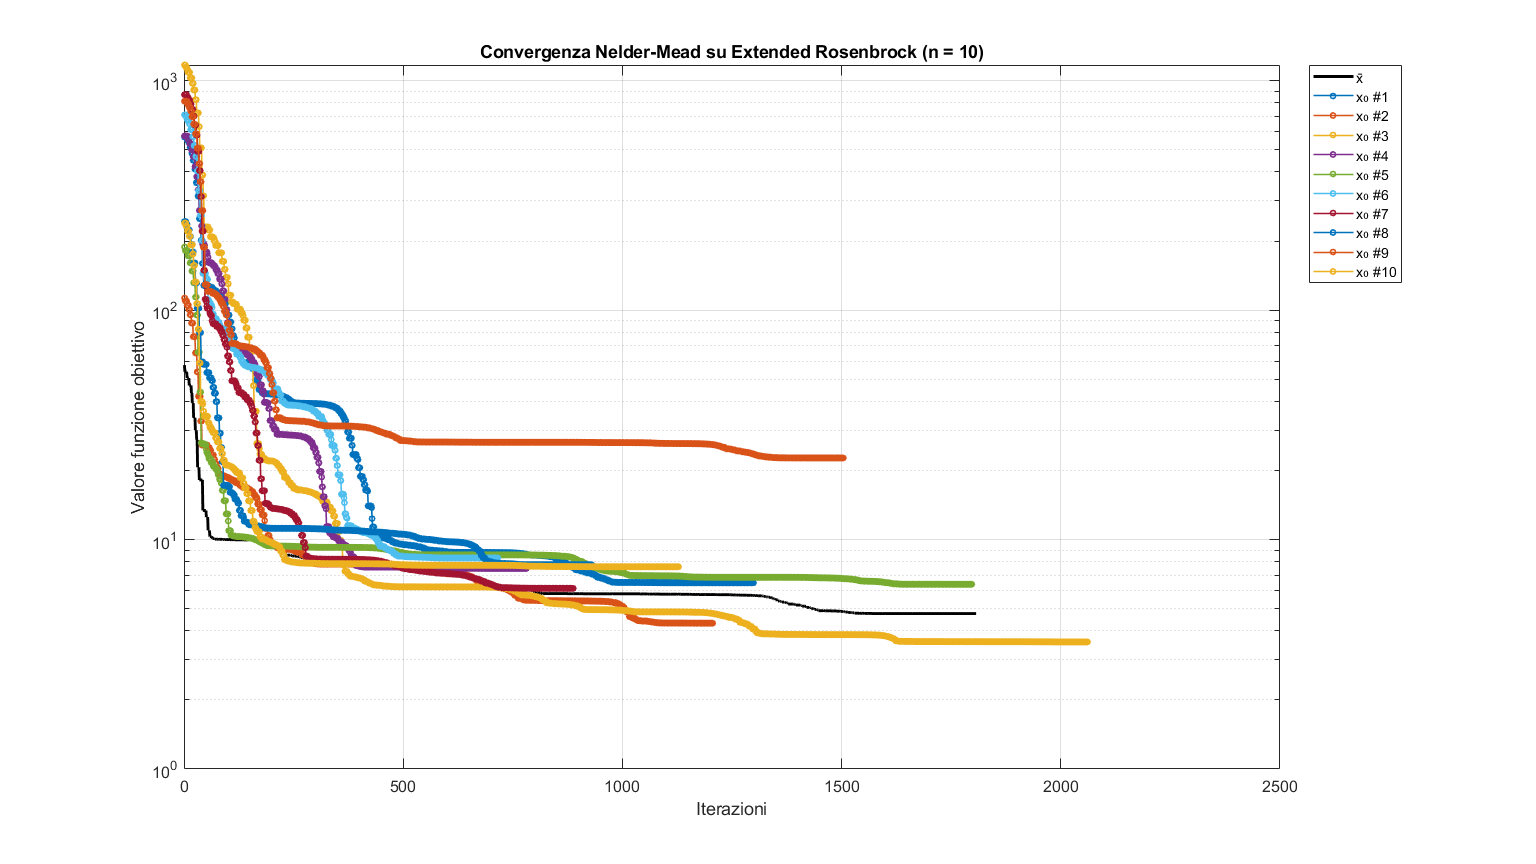
\includegraphics[width=\textwidth]{../immagini/ext_10.png}
		\caption{Convergence of Nelder–Mead on Extended Rosenbrock function ($n=10$) from reference and 10 random initial points. The objective decreases but stagnates above the global minimum.}
		\label{fig:nelder_rosen_10}
	\end{figure}
	
	\begin{figure}[htbp]
		\centering
		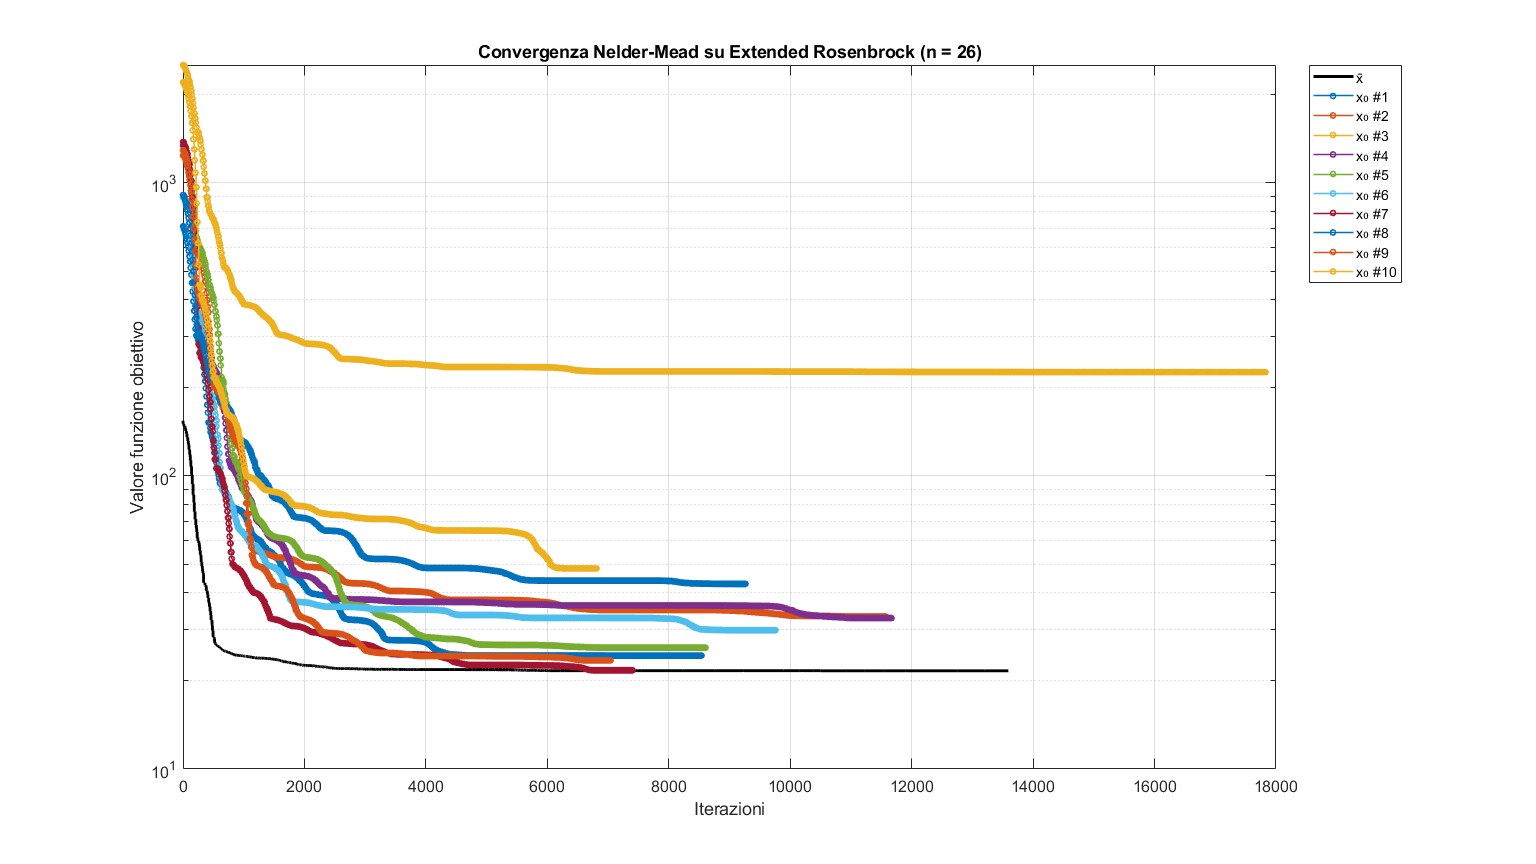
\includegraphics[width=\textwidth]{../immagini/ext_26.png}
		\caption{Convergence of Nelder–Mead on Extended Rosenbrock function ($n=26$). Progress slows down and most trajectories fail to improve after early iterations.}
		\label{fig:nelder_rosen_26}
	\end{figure}
	
	\begin{figure}[htbp]
		\centering
		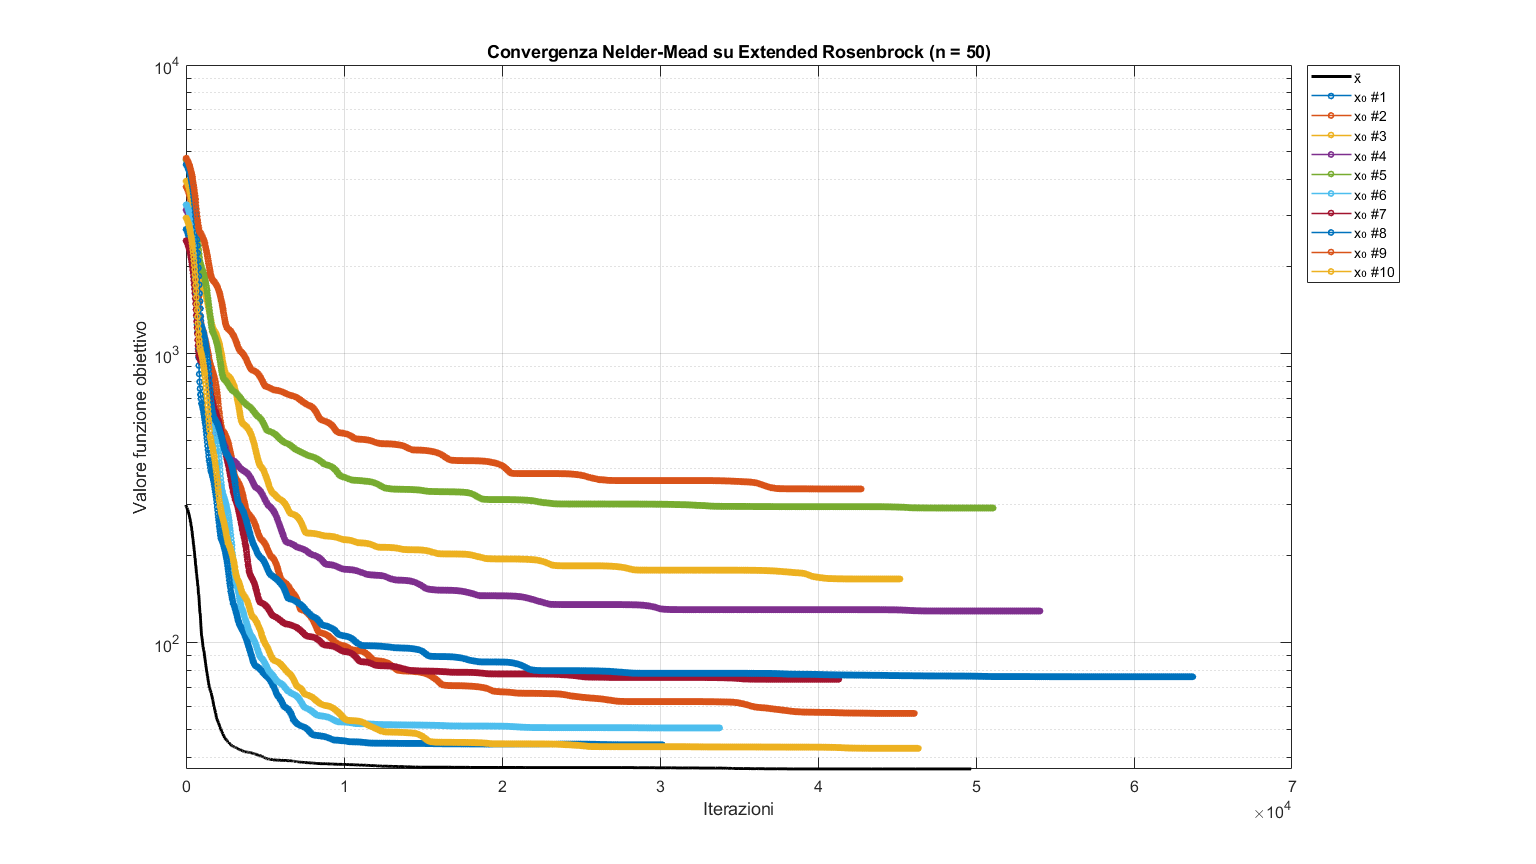
\includegraphics[width=\textwidth]{../immagini/ext_50.png}
		\caption{Convergence of Nelder–Mead on Extended Rosenbrock function ($n=50$). None of the trials reach satisfactory objective values, confirming the method’s limits in high dimensions.}
		\label{fig:nelder_rosen_50}
	\end{figure}
	
	\begin{figure}[htbp]
		\centering
		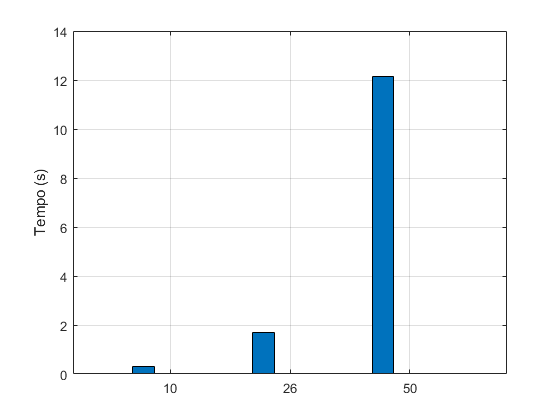
\includegraphics[width=0.6\textwidth]{../immagini/ext_time_nelder.png}
		\caption{Execution time of Nelder–Mead on Extended Rosenbrock for increasing dimensions $n=10$, $26$, and $50$. The cost grows sharply due to the increased simplex size.}
		\label{fig:nelder_rosen_times}
	\end{figure}
	
	\section{Generalized Broyden Tridiagonal Function}
	\subsection{Exact Gradient and Hessian}
	\subsection{Finite Differences Gradient and Hessian}
	
	\section{Banded Trigonometric Function}
	\subsection{Exact Gradient and Hessian}
	\subsection{Finite Differences Gradient and Hessian}
	
	\section{Conclusions}
	
	% -------------------------------------------------
	\appendix              % da qui in poi usa lettere (A, B…)
	% -------------------------------------------------
	\section{Code snippets}
	\subsection{Code for Method Implementations}
	\subsubsection{Modified Newton Method}
	\subsubsection{Truncated Newton Method}
	\subsection{Code for Objective Functions}
	\subsubsection{Rosenbrock Function}
	\subsubsection{Extended Rosenbrock Function}
	\subsubsection{Generalized Broyden Tridiagonal Function}
	\subsubsection{Banded Trigonometric Problem}
	\subsection{Utility Code for Running Experiments}
	
\end{document}
